\documentclass{article}

\usepackage{geometry}
\usepackage{amsmath}     % For aligned environments and advanced math formatting
\usepackage{amssymb}     % For additional math symbols
\usepackage{mathtools}   % Enhances amsmath capabilities
\usepackage{algorithm}
\usepackage{algorithmic}
%\usepackage{algpseudocode}

\usepackage{float}       % For [H] specifier in the algorithm environment
\usepackage{threeparttable} % For footnotes in tables
\usepackage{graphicx}    % For rotating text
\usepackage{adjustbox}   % For adjusting box sizes and positions
\usepackage{subcaption}
\usepackage{xcolor}
\usepackage{multirow}
\usepackage{booktabs}
\usepackage{longtable,microtype,placeins}
\setlength{\emergencystretch}{2em}
\newcommand{\diag}{\operatorname{diag}}
\newcommand{\softplus}{\operatorname{softplus}}
\usepackage{hyperref}
\providecommand{\FloatBarrier}{} % no-op; all floats use [H]

% natbib for arXiv-compatible bibliography
\usepackage[numbers]{natbib}
\renewcommand{\bibname}{References}

% Green editorial suggestions for discussion with colleagues
\newcommand{\greennote}[1]{{\color{green!60!black}\textbf{[Suggestion:} #1\textbf{]}}}

% Extra macros used in appendices (from supplement)
\newcommand{\E}{\mathbb{E}}
\DeclareMathOperator{\tr}{tr}

\geometry{
 a4paper,
 total={170mm,257mm},
 left=20mm,
 top=20mm,
}

\setlength{\parindent}{0pt} % Sets paragraph indentation to 0 points
%\setlength{\parskip}{0.5em}

\newcommand{\norm}[1]{\left\lVert#1\right\rVert}
% \providecommand{\abs}[1]{\left\lvert#1\right\rvert}
\newcommand{\omegaVector}{\boldsymbol{\omega}}
\newcommand{\omegaRV}{\boldsymbol{\Omega}}
\newcommand{\xVector}{\boldsymbol{x}}
\newcommand{\xRV}{\boldsymbol{X}}
\newcommand{\bVector}{\boldsymbol{b}}
\newcommand{\ampl}{a}
\def\BFBH{\boldsymbol{a}}
\newcommand{\rwInc}{\boldsymbol{\nu}}
\newcommand{\cset}{\mathbb{C}}
\newcommand{\C}{\mathbb{C}}
\def\BARS{\mathbf{S}}
\newcommand{\nset}{\mathbb{N}}
\newcommand{\rset}{\mathbb{R}}
\def\R{\mathbb{R}}
\def\E{\mathbb{E}}
\def\BFO{\boldsymbol{\omega}}
\def\DATAM{{\rho}}
\def\rmD{{\mathrm{d}}}
\providecommand{\freqv}{\ensuremath{\boldsymbol{\omega}}}
\providecommand{\freq}{\ensuremath{\omega}}
\DeclareMathOperator*{\argmax}{arg\,max}
\DeclareMathOperator*{\argmin}{arg\,min}
\def\Ll{\mathcal{L}}
\def\ID{\mathbf{I}}
\def\IM{\mathrm{i}}
\providecommand{\weightv}{\ensuremath{\hat{\boldsymbol{\beta}}}}
\providecommand{\weight}{\ensuremath{\hat{\beta}}}
\providecommand{\T}{\mathrm{T}}    % Transpose symbol
\def\ALPHAEX{\gamma}             % what used to be exponent
\providecommand{\algAM}{\ensuremath{\mathrm{AM}}}
\providecommand{\algAMR}{\ensuremath{\mathrm{AMR}}}
\providecommand{\algAMRmod}{\ensuremath{\mathrm{AMRv2}}}
\providecommand{\algRWR}{\ensuremath{\mathrm{RWR}}}

\title{Two-Stage Drift and Covariance Regression for SDE Learning
with Adaptive Random Fourier Features}
\author{Owen Douglas, Aku Kammonen, Anamika Pandey, Raul Tempone }
\date{Review draft --- September 2026; author decisions remain open}

\begin{document}

\maketitle

\begin{abstract}
Learning stochastic dynamics from limited observations is a central challenge in data-driven modelling of It\^{o} SDEs. We present a sequential procedure for estimating drift and diffusion covariance from snapshot triples $(x_0,x_1,h)$. Conditional first and second moments of the short-time Gaussian model motivate two multi-output Fourier-feature regressions with closed-form ridge amplitude solves and adaptive frequencies. Out-of-fold drift predictions construct covariance targets, while validation selects each retained model. Restricted ridge regression is not an exact decomposition of joint finite-sample likelihood optimization. Applications include polynomial systems, a stochastic SIR mean-field limit, a wave-derived regression, broad-spectrum drift and near-singular covariance. Historical-protocol examples provide validation-selected evidence; a corrected near-singular benchmark compares five approximately parameter-matched estimators on independent test observations. ARFF has the smallest raw covariance error there, but joint MLP has substantially smaller drift error and neural alternatives achieve lower Gaussian negative log-likelihood. Raw covariance validity and projected likelihood are reported separately. Completed sample-size, lag and capacity studies characterize sensitivity without establishing universal convergence rates or speed advantages.

\end{abstract}



\section{Introduction}
Identifying stochastic dynamics from limited and noisy observations is a central challenge across science and engineering. Stochastic differential equations (SDEs) provide flexible models for noisy, multiscale systems in physics \cite{risken1996fokker,vankampen2007stochastic}, finance \cite{Yacine_finance,james2000interest}, and biology \cite{Schwartz_biology}.

\textcolor{black}{Classical statistics for discretely observed diffusions provides maximum-likelihood approximations, estimating functions, Bayesian methods, and nonparametric coefficient estimators \citep{Yacine_finance,Sorensen2009}. These methods are powerful, but often require model-specific transition-density approximations, asymptotic regimes, or nontrivial numerical integration. Our setting emphasises scattered snapshot triples, flexible multivariate covariance regression, and computational training through adaptive random features.}

Penalized nonparametric least-squares coefficient estimation already has a classical foundation: Comte, Genon-Catalot and Rozenholc \citep{Comte2007} study regularly sampled stationary one-dimensional diffusions and data-driven finite-dimensional spaces. Their risk results do not transfer automatically to adapted multivariate Fourier models or our finite-lag snapshots. Sequential moment regression itself is not a novelty claim.

Recent machine learning approaches aim to relax these limitations by fitting drift and diffusion directly from data.
Neural SDEs \cite{neural_SDEs} and SDE-Net \cite{SDE_Net} parametrise the coefficients with neural networks, while \cite{Dietrich2023,dridi2021learningstochasticdynamicalsystems} proposed likelihood-based training under Euler--Maruyama discretisation.
Gaussian-process coefficient learning with data-adapted kernels has also been explored \cite{Darcy2023}, and neural SDE variants \cite{neural_SDEs,SDE_Net,Dietrich2023,dridi2021learningstochasticdynamicalsystems} are promising; however, neural networks typically rely on gradient-based training (e.g., Adam \citep{kingma2017adammethodstochasticoptimization}), which motivates seeking a simpler alternative.

Random Fourier features (RFF) \cite{RR2007RandomFF,Li2021UnifiedRFF} offer a contrasting approach:
functions are represented with randomised trigonometric bases, and training reduces to closed-form least squares.
Recent works have further advanced the theoretical understanding and extensions of RFF:
Szabó \& Sriperumbudur study derivative approximations via RFF~\citep{pmlr-v89-szabo19a},
Li et al.\ propose quadrature-based Fourier features for scalable Gaussian process regression~\citep{pmlr-v238-li24o},
and Yao et al.\ introduce bootstrap error estimation techniques for RFFs~\citep{pmlr-v206-yao23a}.
Adaptive variants (ARFF) \cite{kammonen2020adaptiverandomfourierfeatures,Kammonen2025Adaptive,huang2025convergenceadaptiveresamplingrandom}
adapt frequency populations through random-walk proposals and optional resampling, motivated by population Fourier approximation bounds. The ARFF approach was first proposed in \cite{kammonen2020adaptiverandomfourierfeatures}, where the Fourier frequencies are adapted using a Metropolis-based sampling. This built upon earlier RFF works such as  \cite{RR2007RandomFF, NIPS2008RR, Barron1993, Barron1994}, where authors attempted to identify optimal frequency sampling distributions or feature weights. Later, \cite{Kammonen2025Adaptive} enhanced this idea by adding a resampling step, inspired by particle-filtering, whose published experiments study sensitivity to proposal lengths and acceptance exponents; this does not establish a uniform benefit in SDE regression.
 \textcolor{black}{The present manuscript substantially revises and extends our earlier ARFF-for-SDE-learning preprint~\cite{douglas2025arffsde} by sharpening the drift–diffusion split, adding near-singular covariance diagnostics, and expanding the empirical analysis.}



% Our key idea is that the Gaussian negative log-likelihood induced by Euler--Maruyama discretisation admits a decomposition into two regression problems: one for drift increments and one for diffusion covariances.
% This reduction allows us to replace backpropagation-based training with ARFF loops consisting only of resampling, random-walk updates in frequency space, and closed-form least-squares solves---yielding a simple alternative to gradient descent for learning SDEs from snapshot data. \greennote{Importantly, we observe experimentally that the benefits of this decomposition are not tied to the ARFF optimiser itself: even when trained with the same optimiser (Adam), the split formulation can improve training behavior compared with direct optimisation of the joint likelihood.}
%  {\color{red}the green suggestion is good but above need some rewording:}\\
% {\color{black}Our key idea is that, for the Gaussian negative log-likelihood induced by Euler--Maruyama discretisation, fixing the diffusion reduces the loss to a least-squares regression for the drift, and the resulting pointwise likelihood minimisers for the diffusion provide regression targets for learning the diffusion covariance.
This sequential formulation makes the two coefficient-learning tasks explicit. For fixed frequencies, all output amplitudes are fitted jointly in a linear ridge solve, confining nonlinear search to the frequency population. The drift stage does not invert a learned covariance, and the second stage estimates covariance entries rather than a nonunique diffusion factor. These conveniences do not eliminate noisy-target variance, feature conditioning or raw covariance indefiniteness.

\paragraph{Contributions}
(i) We derive the unrestricted conditional targets induced by the Gaussian observation model and distinguish them from the restricted regression surrogates.
(ii) We implement a two-stage ARFF procedure with out-of-fold covariance targets, validation-selected checkpoints and explicit raw-covariance/likelihood evaluation.
(iii) We provide operation counts and applications to polynomial, epidemic, spectrally broad and wave-derived systems, retaining their actual protocols and mixed outcomes.
(iv) We compare joint and split Adam with ARFF on a corrected near-singular benchmark and report completed descriptive sensitivity studies. These compare complete estimators; they do not isolate a causal advantage of frequency adaptation or establish universal speed, accuracy or convergence-rate superiority.

\paragraph{Paper outline}
Section~\ref{sec:ARFFalgorithm_updating} reviews ARFF.
Section~\ref{sec:mathprobset} formulates the likelihood-based learning problem,
and Section~\ref{sec:training_algorithm} presents the proposed ARFF training procedure.
Section~\ref{sec:computational_experiments} describes the benchmark setup,
and Section~\ref{sec:results} reports the experimental results.
Section~\ref{sec:summary} concludes with a discussion of findings and future directions.
Experiment specifications are provided in Appendix~\ref{app:num_experiments}, and reproducibility information in Appendix~\ref{app:reproducibility}.


\section{Adaptive Random Fourier Features Training Algorithm}
\label{sec:ARFFalgorithm_updating}

Consider the data $(x_n, y_n)\in\mathbb{R}^D\times\mathbb{R}^{D'},\qquad n=1,\dots,N,$
where the inputs $x_n$ are drawn i.i.d.\ from an unknown population distribution $\rho$, and there exists a target function $g:\mathbb{R}^D\to\mathbb{R}^{D'}$ such that $y_n=g(x_n) + \xi_{n},$ where $\xi_{n}$ denotes possible measurement noise. Fourier feature models approximate a target function $g$ by representing it in the finite-dimensional space
\[
\mathcal N_K=\{\beta(x)=\Phi_\Omega(x)B:\ B\in\mathbb R^{2K\times D'}\},\quad
\Phi_\Omega(x)=[\cos(x\Omega),\sin(x\Omega)].
\]
For a fixed set of frequencies $\{\omega_k\}_{k=1}^K$, the coefficients $\hat{\beta}_k$ are obtained by solving a regularised least-squares problem, producing an empirical approximation $\beta \approx g$. At the population level this is
\begin{equation}
\label{eq:regularised_loss}
\min_{\beta\in\mathcal{N}_K}
\Bigl\{\,
\E_{\rho}[\,\|y-\beta(x)\|^2\,]
\,+\,
\lambda\|B\|_F^2
\Bigr\},
\end{equation}
where $\lambda>0$ is a Tikhonov regularisation parameter and $\|\cdot\|$ denotes the Euclidean norm. In practice one minimises its empirical version, which is attained by replacing $\rho$ with $\hat{\rho}$ which denotes the empirical distribution of $\{(x_n, y_n)\}_{n=1}^N$.

\paragraph{Optimal sampling density}
The population random-feature analysis motivates frequency adaptation. Under the scalar theorem's integrability and spectral-moment assumptions, iid frequencies with density $p$ obey \citep[Theorem 2.1]{kammonen2020adaptiverandomfourierfeatures}
\[
\E_{\omega_{1:K}}\min_\beta\{\E|\beta(X)-Y|^2+\lambda\|\hat\beta\|^2\}
\le \frac{1+\lambda}{K}\E_{\omega\sim p}\frac{|\widehat g(\omega)|^2}{(2\pi)^D p(\omega)^2}
+\E|Y-g(X)|^2.
\]
The spectral term is minimized by $p_*(\omega)\propto|\widehat g(\omega)|$ when defined; pooling vector outputs motivates the corresponding norm. This is a frequency-averaged population result, including irreducible noise, not a guarantee for a finite-data, adapted and validation-selected estimator. The ideal density motivates proposals; convergence of the implemented population to it is not asserted.

For a fixed frequency population, real multi-output amplitudes solve
\begin{equation}\label{eq:normal_equations_ARFF}
 (S^\top S+n\lambda I)B=S^\top Y,\qquad S_{i,:}=\Phi_\Omega(x_i),
\end{equation}
where $n$ is the actual fitting subset size and $S$ has $2K$ unnormalized columns, ordered cosine block then sine block. This minimizes $n^{-1}\|SB-Y\|_F^2+\lambda\|B\|_F^2$. It is not asserted equivalent to unconstrained complex regression followed by taking real parts.

The Metropolis-inspired procedure \citep{kammonen2020adaptiverandomfourierfeatures} favors proposals with larger pooled amplitudes; optional resampling \citep{Kammonen2025Adaptive} redistributes frequency slots. The noisy-data convergence analysis \citep{huang2025convergenceadaptiveresamplingrandom} includes quadratic and quartic penalties and separate assumptions; it does not directly certify the ridge-only procedure here. Algorithm~\ref{alg:ARFF} specifies modern Experiment 8. Historical applications retain the distinct stopping/resampling rules in Appendix~\ref{app:reproducibility}.

\begin{algorithm}[H]\small
\caption{Modern validation-selected ARFF regression (Experiment 8)}\label{alg:ARFF}
\textbf{Input:} regression pool $(x_i,y_i)$; $K,\lambda,\delta,\gamma$, 300 adaptations.
\begin{enumerate}
\item Split the pool into a seeded 10\% internal validation set $V$ and fitting set $F$. All amplitude solves use only $F$ and $n=|F|$ in \eqref{eq:normal_equations_ARFF}. Initialize frequencies at zero and solve amplitudes. Positive ridge makes this repeated-feature amplitude problem well-defined in exact arithmetic; the first random proposals diversify frequencies. This is not a guarantee of numerical conditioning in finite precision.
\item At each adaptation propose $\omega'_k=\omega_k+\delta Z_k$, $Z_k\sim\mathcal N(0,I_D)$, and solve proposed amplitudes $B'$ jointly. Define
\[
a_k=\left(\sum_{j=1}^{D'}(B_{kj}^2+B_{K+k,j}^2)\right)^{1/2},\quad
\bar a_k=\max(a_k,\tau),\quad\bar a'_k=\max(a'_k,\tau),
\]
where $\tau$ is the amplitude dtype's smallest positive normal number. Accept each proposed frequency \emph{with probability}
$\alpha_k=\min\{1,(\bar a'_k/\bar a_k)^\gamma\}$: the code compares the ratio to an independent uniform $U_k\in[0,1)$. Guarding both norms makes two zero norms give ratio one.
\item Refit amplitudes for the accepted/rejected mixed frequency population on $F$. Compute $\operatorname{MSE}_V=(|V|D')^{-1}\sum_{i\in V}\|\Phi_\Omega(x_i)B-y_i\|^2$ and retain the first strict minimum.
\item Return the selected model with no post-selection refit. Only post-adaptation iterations 1--300 are candidates; nonfinite losses become infinity and a fit without a finite candidate fails.
\end{enumerate}
The baseline uses $K=128,\lambda=.001,\delta=.2,\gamma=1$, Metropolis on and resampling off. $M_{\min}=M_{\max}=300$ disables early stopping.
\end{algorithm}

\section{Mathematical Problem Setting}\label{sec:mathprobset}
This work aims to identify an SDE model that approximates the observed dynamics of a system from one-step transition data (snapshot triples $(x_0,x_1,h)$).
 The assumed form of the SDE is an It\^{o} diffusion process
\begin{equation}
\label{eq:ito diffusion SDE}
    \mathrm{d}x_t = f(x_t) \, \mathrm{d}t + \sigma(x_t) \, \mathrm{d}W_t,
\end{equation}
where $x_t \in \mathbb{R}^D$ is the system state at time $t$, $f: \mathbb{R}^D \to \mathbb{R}^D$ is the drift function, and $\sigma: \mathbb{R}^D \to \mathbb{R}^{D \times m}$ is the diffusion factor. These functions are assumed to satisfy appropriate regularity conditions (see Chapter~5 in \cite{BerntSDE}) that ensure the existence of a solution to Eq.~\eqref{eq:ito diffusion SDE}.
 The process $W_t$ is an $m$-dimensional Wiener process with independent increments, such that $W_{t} - W_{s} \sim \mathcal{N}(0, (t-s)I_m)$ for $0\leq s < t$.

Training data consist of finite-lag transitions of the system, in the form $\mathcal{D} = \{(x_0^{(n)}, x_1^{(n)}, h^{(n)})\}_{n=1}^N,$
where $x_0^{(n)}$ is the initial point and $x_1^{(n)}$ the state after a small time increment $h^{(n)} > 0$.

\begin{center}\small
\begin{tabular}{ll}
$D,m$ & state and driving-noise dimensions\\
$h,\Delta t$ & observation lag and fine integration step\\
$f,\sigma,\Sigma$ & drift, diffusion factor, covariance $\sigma\sigma^\top$\\
$K,2K,q$ & frequency count, real feature count, regression output count\\
$\lambda,\varepsilon$ & amplitude ridge penalty, scoring eigenvalue floor
\end{tabular}
\end{center}
\subsection*{Euler--Maruyama Approximation and Transition Density}

Using the Euler--Maruyama (EM) scheme, the forward evolution of the SDE over a time step $h>0$ can be approximated as $x_1 \approx x_0 + h f(x_0) + \sigma(x_0)\,\delta W$, $\delta W \sim \mathcal{N}(0, h I_m).$
Consequently, the conditional distribution of $x_1$ given $x_0$ and $h$ is approximated by $x_1 \mid x_0,h \approx \mathcal{N}\!\big(x_0 + h f(x_0),\, h\Sigma(x_0)\big)$,
where $\Sigma(x_0) = \sigma(x_0)\sigma(x_0)^\top\succeq0$.
This law is exact for a frozen one-step EM update. For the multiple-substep SDE observations used here it is a Gaussian quasi-likelihood, not an exact transition density.

\subsection*{Learning Objective}

We introduce real Fourier models $f_\theta(x)=\Phi_\Omega(x)B_f$ and $\widehat\Sigma_{\theta'}(x)=\Phi_{\Omega'}(x)B_\Sigma$. The second output is the lower-triangular vectorization of covariance (or its diagonal in diagonal experiments); reversing this vectorization gives a symmetric matrix, not a guarantee of positive definiteness. For full covariance there are $q=D(D+1)/2$ outputs. Frequencies and amplitudes of drift and covariance are distinct.

Following \cite{Dietrich2023,dridi2021learningstochasticdynamicalsystems},
the negative log-likelihood for one sample, on coordinates where $\Sigma_{\theta\prime}(x_0)$ is positive definite, is
\begin{equation}
\label{eq:loss}
    \mathcal{L}(\theta, \theta' \mid x_0, x_1, h) =
    \frac{1}{2} (x_1 - x_0 - h f_\theta(x_0))^\top (h\Sigma_{\theta'}(x_0))^{-1} (x_1 - x_0 - h f_\theta(x_0))
    + \frac{1}{2} \log|h\Sigma_{\theta'}(x_0)| + \frac{D}{2} \log(2\pi).
\end{equation}
where $\|v\|^2_{M} := v^\top M v$ for any symmetric positive definite matrix $M$ and $\log|\cdot|$ denotes the log-determinant.
For a degenerate frozen update, this full-state density does not exist: score the relevant stochastic coordinates with positive definite covariance, or explicitly use a regularized Gaussian scoring model. Eigenvalue flooring defines such a scoring model; it does not recover the true transition law.
The population loss is
\begin{equation}
\label{eq:total_loss}
\mathcal{L}_{\text{pop}}(\theta, \theta')
= \E_{\rho}\!\big[\mathcal{L}(\theta,\theta' \mid x_0,x_1,h)\big],
\end{equation}
with $\rho$ the true distribution of snapshot triples.
For joint likelihood training, $\rho$ is unknown and we minimise the empirical loss
$\mathcal{L}_{\text{emp}}$ obtained by replacing $\rho$ with the
empirical distribution $\hat{\rho}$ of $\mathcal{D}$. Section~4 instead defines sequential regression surrogates.

Minimisation with respect to the diffusion $\sigma$ is equivalent
to minimisation over the covariance $\Sigma=\sigma\sigma^\top$ only when the covariance class is exactly the image of the factor class.
Since the mapping $\sigma \mapsto \Sigma$ is many-to-one, structural
assumptions are required for identifiability. For example, the SPD principal square root is one convention, while a lower-triangular factor with positive diagonal is fixed by Cholesky decomposition. Symmetry alone does not identify the principal root.

\textcolor{black}{Throughout the manuscript, $\sigma$ denotes a diffusion factor and
$\Sigma=\sigma\sigma^\top$ denotes the associated covariance.
Algorithm~\ref{alg:ARFF_SDE} learns $\Sigma$ directly through
residual covariance targets. Whenever errors or visualizations are
reported, we state explicitly whether the quantity shown is
$\sigma$ or $\Sigma$.}

\section{Drift and Diffusion Training Algorithm}\label{sec:training_algorithm}







{\color{black}
This section presents the proposed drift and diffusion training
procedure. Under the Gaussian Euler--Maruyama observation model, the
drift and diffusion covariance are characterised by the conditional
mean of the scaled increments and the conditional second moment of the
residuals, respectively. These identities motivate the regression
surrogates used in Alg.~\ref{alg:ARFF_SDE}.
}

For a symmetric matrix $A$, the relation $A \succ 0$ means $A$ is  positive definite, and $A \succeq 0$ means positive semidefinite. For a vector $v$ and $M \succ 0$, we write $\|v\|_M^2 := v^\top M v$.

\subsection{Drift learning objective}
\label{sec:drift_reduction}


{\color{black}
This subsection derives the population drift target induced by the
Gaussian Euler--Maruyama likelihood and relates it to the regression
surrogate used in Alg.~\ref{alg:ARFF_SDE}.

Conditionally on $x_0=x$, assume $h>0$ almost surely, $0<\E[h\mid x]<\infty$, $\E[\|x_1-x_0\|^2/h\mid x]<\infty$ and $\E[|\log h|\mid x]<\infty$. These make the pointwise Gaussian objective finite for each finite drift and SPD covariance. Statements about an integrated population loss additionally require these conditional terms to be integrable over $x$. For the unweighted increment identity require $\E[\|(x_1-x_0)/h\|\mid x]<\infty$, for example finite $\E[h^{-1/2}\mid x]$ in the frozen Gaussian model.

Assume that the fixed covariance field satisfies
\[
\Sigma_{\tilde\theta'}(x)\succ0
\]
for all $x$ (or almost surely with respect to $\rho$).

Define
\[
y:=\frac{x_1-x_0}{h},
\qquad
A(x):=\Sigma_{\tilde\theta'}(x)^{-1}.
\]

For fixed diffusion parameters $\theta'=\tilde\theta'$, the quadratic part
of the population negative log-likelihood is
\[
Q(f)
=
\frac12
\E_{\rho}\!\left[
h\,(y-f(x_0))^\top
A(x_0)
(y-f(x_0))
\right].
\]

Since $A(x_0)\succ0$ almost surely, the unrestricted minimiser satisfies
\[
f^*(x)
=
\frac{\E_{\rho}[hy\mid x_0=x]}
     {\E_{\rho}[h\mid x_0=x]}.
\]

If \(h\) is deterministic, or if the conditional expectation
\[
\E_{\rho}[y\mid x_0=x,\,h]
\]
is independent of \(h\), then
\[
f^*(x)=\E_{\rho}[y\mid x_0=x].
\]

Under the frozen-coefficient one-step Euler--Maruyama model,
\[
\E_{\rho}[y\mid x_0=x,h]=f(x),
\]
and therefore
\[
f^*(x)=f(x).
\]

Thus, under the Euler--Maruyama observation model, the weighted and
unweighted population targets coincide.
}



\paragraph{Squared-loss moment scope}
Population squared-loss regression additionally requires $\E\|Y\|^2<\infty$, where $Y=(x_1-x_0)/h$. For the covariance target $T=rr^\top/h$, conditional on the fitted nuisance model, require $\E[\|T\|_F^2\mid\mathcal G]=\E[\|r\|^4/h^2\mid\mathcal G]<\infty$ (and integrability over $\mathcal G$ if averaging fitted models). Lower-triangle vectorization has equivalent finiteness. These are separate assumptions from likelihood integrability and the first-moment identity; no new convergence assertion for all applications follows.

{\color{black} \paragraph{Empirical surrogate}
Motivated by the unweighted conditional-mean identity under the frozen Euler--Maruyama model, we fit the following ordinary ridge surrogate. It differs from the empirical fixed-covariance likelihood objective displayed below:
\[
\min_{f\in\mathcal N_K}
\left\{
\frac{1}{N}
\sum_{n=1}^{N}
\left\|
Y_n-f(x_0^{(n)})
\right\|_2^2
+
\lambda
\sum_{k=1}^{K}
\|\hat{\beta}_k\|_2^2
\right\},
\]
where
\[
Y_n=\frac{x_1^{(n)}-x_0^{(n)}}{h_n}.
\]

This objective is not, in general, the exact finite-sample minimizer
of the Gaussian negative log-likelihood.

\paragraph{Exact fixed-covariance likelihood.}
For fixed covariance parameters $\theta'=\tilde\theta'$, the exact
finite-sample Gaussian likelihood yields the generalized least-squares
problem
\[
\min_{f\in\mathcal N_K}
\left\{
\frac1N
\sum_{n=1}^{N}
h_n
\bigl(
Y_n-f(x_0^{(n)})
\bigr)^\top
\Sigma_{\tilde\theta'}(x_0^{(n)})^{-1}
\bigl(
Y_n-f(x_0^{(n)})
\bigr)
+
\lambda
\sum_{k=1}^{K}
\|\hat\beta_k\|_2^2
\right\}.
\]

Thus, the exact finite-sample likelihood corresponds to a
covariance-weighted generalized least-squares problem, whereas
Algorithm~\ref{alg:ARFF_SDE} employs ordinary ridge regression.
Under the frozen Euler--Maruyama model the unrestricted targets agree; restricted regularized solutions need not. For feature columns $\phi_n$ and $W_n=h_n\Sigma(x_n)^{-1}$, the displayed penalized GLS objective satisfies
\[
\sum_n\phi_n\phi_n^\top B W_n+N\lambda B=\sum_n\phi_nY_n^\top W_n.
\]
Ordinary ridge replaces the weights with identity matrices. This distinction remains even when the population drift identity is exact.
}

\subsection{Diffusion minimiser: pointwise characterisation and plug-in targets}
\label{sec:diffusion_minimiser}

Fix $x_0 \in \R^D$ and a drift $f_\theta$. For one observation $(x_1,h)$, define the residual
\[
r := x_1 - x_0 - h\,f_\theta(x_0).
\]
As a function of the covariance $\Sigma \in \R^{D\times D}$ with $\Sigma \succ 0$, the (centered) negative log-likelihood contribution is
\begin{equation}
\label{eq:diff_ll_single}
\ell(\Sigma; x_0, x_1, h)
= \tfrac{1}{2}\, r^\top (h \Sigma)^{-1} r \;+\; \tfrac{1}{2}\,\log|h \Sigma| \;+\; \mathrm{const}.
\end{equation}
Conditioning on $x_0$ and taking expectation over $(x_1,h)\mid x_0$ yields the pointwise population objective
\begin{equation}
\label{eq:diff_obj_pointwise}
\mathcal{L}(\Sigma; x_0)
= \tfrac{1}{2}\,\tr\!\big(\Sigma^{-1} C(x_0)\big) \;+\; \tfrac{1}{2}\,\log|\Sigma| \;+\; \mathrm{const},
\qquad
C(x_0) := \E\!\left[h^{-1} r r^\top \mid x_0\right].
\end{equation}



{\color{black}
Let
\[
\mathbb S_{++}^{D}
:=
\{A\in\mathbb R^{D\times D}:
A=A^\top,\;
A\succ0\}
\]
denote the set of symmetric positive definite matrices.

\paragraph{Proposition (Pointwise minimiser and uniqueness)}
Assume $C(x_0)\succ0$. Consider
\[
\mathcal{L}(\Sigma;x_0)
=
\frac12\tr\!\bigl(\Sigma^{-1}C(x_0)\bigr)
+
\frac12\log\det\Sigma,
\qquad
\Sigma\in\mathbb S_{++}^D.
\]
Under the precision parametrisation $P=\Sigma^{-1}$, define
\[
\widetilde{\mathcal L}(P;x_0)
:=
\mathcal L(P^{-1};x_0)
=
\frac12\tr\!\bigl(PC(x_0)\bigr)
-
\frac12\log\det P,
\qquad
P\in\mathbb S_{++}^D.
\]
The function $\widetilde{\mathcal L}(P;x_0)$ is strictly convex in
$P$. Consequently, its unique minimiser is
\[
P^*=C(x_0)^{-1},
\]
and the unique covariance minimiser is
\[
\Sigma^*(x_0)=C(x_0).
\]

\emph{Proof.}
The mapping $\Sigma\mapsto P=\Sigma^{-1}$ is a bijection on
$\mathbb S_{++}^D$. Hence minimising
$\mathcal L(\Sigma;x_0)$ over $\Sigma\in\mathbb S_{++}^D$
is equivalent to minimising
$\widetilde{\mathcal L}(P;x_0)$ over
$P\in\mathbb S_{++}^D$.

The term $P\mapsto\tr(PC(x_0))$ is linear, while
$P\mapsto-\log\det P$ is strictly convex on
$\mathbb S_{++}^D$
\citep{boyd2004convex}.
Therefore $\widetilde{\mathcal L}(P;x_0)$ is strictly convex.

Its gradient is
\[
\nabla_P\widetilde{\mathcal L}(P;x_0)
=
\frac12C(x_0)-\frac12P^{-1},
\]
where $P$ is symmetric. The unique stationary point satisfies
\[
P^{-1}=C(x_0),
\]
and therefore
\[
P^*=C(x_0)^{-1}.
\]
Returning to the covariance variable gives
\[
\Sigma^*(x_0)=C(x_0).
\]
\hfill$\square$
}





{\color{black}\paragraph{Remark on singular conditional covariance}
If $C(x_0)\succeq0$ is singular, the objective generally has no
finite minimiser over $\mathbb S_{++}^D$. Indeed, covariance
eigenvalues corresponding to null directions of $C(x_0)$ may approach
zero without increasing the trace term, while the log-determinant term
tends to $-\infty$. A well-posed SPD estimate therefore requires an
eigenvalue floor, ridge regularisation, or an appropriate structural
constraint.

For example, one may regularise the target by
\[
C_\varepsilon(x_0)=C(x_0)+\varepsilon I,
\qquad \varepsilon>0,
\]
or constrain the admissible covariance matrices by
\[
\Sigma-\varepsilon I\succeq0.
\]}


{\color{black} \paragraph{Empirical targets and ARFF regression}
In data, each $x_0^{(n)}$ is typically observed once. We therefore
define the plug-in residual target
\[
\Sigma^{*}_{(n)}
:=
h_n^{-1}r_nr_n^\top,
\qquad
r_n
=
x_1^{(n)}-x_0^{(n)}
-h_nf_\theta\!\bigl(x_0^{(n)}\bigr).
\]
For a fitted drift held fixed under its nuisance-training sigma-field $\mathcal G$ and conditionally independent of the evaluated observation, the target estimates the residual conditional moment (not necessarily the true instantaneous covariance):
\[
\E\!\left[\Sigma^{*}_{(n)}\mid x_0^{(n)},\mathcal G\right]
=
C_{f_\theta}(x_0^{(n)}\mid\mathcal G).
\]
In the implemented procedure each target uses a drift model fitted and selected without that observation's fold. For iid snapshots this supports conditioning on the fitted nuisance model; dependent trajectories or grid observations require additional independence assumptions. Cross-fitting does not remove drift error or finite-lag bias.}

Since Alg.~\ref{alg:ARFF} handles vector outputs, we vectorise by stacking the lower--triangular entries:
\[
\widehat{\Sigma}^{*}_{(n)} \in \R^{q}, \quad q = D(D{+}1)/2.
\]
With a Fourier-feature hypothesis class $\mathcal{N}_{K'}$ for each component and Tikhonov parameter $\lambda_\Sigma \ge 0$, we solve the (decoupled) ridge regressions
\[
\min_{\widehat\Sigma_{\theta'} \in \mathcal{N}_{K'}} \;
\left\{\frac{1}{N}\sum_{n=1}^{N} \Big\| \widehat{\Sigma}^{*}_{(n)} - \widehat{\Sigma}_{\theta'}\!\bigl(x^{(n)}_0\bigr) \Big\|^2
\;+\; \lambda_\Sigma \sum_{k=1}^{K'} \|\hat\beta'_k\|^2\right\},
\]
followed by reconstruction of the symmetric matrix $\Sigma_{\theta'}(x)$ from its vectorised form.

\paragraph{Structural parametrisations}
Direct entry regression is distinct from fitting an SPD factor by Gaussian NLL. Unweighted lower-triangular regression counts an off-diagonal once, whereas full Frobenius error counts it twice. Neither is a restricted-class likelihood projection in general. Adam baselines use their specified diagonal/factor covariance constructions; ARFF reconstructs raw covariance entries and applies the explicit evaluation projection below only where needed.

\paragraph{Drift--diffusion coupling}
Let $\mathcal G$ be the sigma-field generated by a fitted nuisance model $g$ and its training information. Assume an evaluated observation is independent of $\mathcal G$ conditional on $x_0=x$, with the preceding integrability conditions. For the frozen one-step law, $r=h(f-g)(x)+\sqrt h\sigma(x)\xi$ gives
\[
\E[h^{-1}rr^\top\mid x,\mathcal G]
=\Sigma(x)+\E[h\mid x,\mathcal G](f-g)(x)(f-g)(x)^\top.
\]
Cross-fitting is a sample-separation device used more broadly in nuisance estimation \citep{chernozhukov2018}; we do not invoke a double-machine-learning theorem for this estimator. The independence assumption yields $\E[h\mid x,\mathcal G]=\E[h\mid x]$. For fixed lag the coefficient is $h$. Averaging over fitted models averages their error outer products, not only their mean error. Finite-lag observations introduce transition-moment bias as well; cross-fitting removes same-observation fitting but does not by itself eliminate dependence in trajectory or wave-grid data. Residual outer products are PSD of rank at most one, not generally SPD.

Alg.~\ref{alg:ARFF_SDE} summarises the resulting two-stage training procedure.

\begin{algorithm}[H]\small
\caption{Two-stage ARFF SDE learning with five-fold cross-fitting}\label{alg:ARFF_SDE}
\textbf{Input:} outer-training triples, partitioned into five fixed folds $I_k$.
\begin{enumerate}
\item For each fold $I_k$, fit and select a drift model $f^{(-k)}$ on the other four folds using Algorithm~\ref{alg:ARFF}, with targets $(x_1-x_0)/h$. Predict only the excluded fold.
\item For each training row $n$, form $r_n=x_{1,n}-x_{0,n}-h_nf^{(-k(n))}(x_{0,n})$ and $T_n=\operatorname{vec}_\ell(r_nr_n^\top/h_n)$ (diagonal entries for diagonal models).
\item Fit a separate final drift model on the full outer-training pool and a covariance model on that pool with targets $T_n$. Each call still uses Algorithm~\ref{alg:ARFF}'s internal holdout: ``full training pool'' does not mean amplitudes use every row. There is no post-selection refit.
\item Freeze selected models, then evaluate. Use raw covariance for coefficient RMSE and raw-SPD diagnostics; symmetrize and floor eigenvalues where SPD covariance is required for NLL.
\end{enumerate}
There are seven regressions. At baseline Ex8 $N_{\rm train}=80000$, final amplitude fits use 72000 rows and each nuisance fit 57600. Historical applications replace the inner adaptation/stopping loop by their documented compatibility variant, while retaining OOF targets.
\end{algorithm}

\subsection{Split vs joint training}
\label{sec:split_vs_joint}

Existing SDE learning approaches employ joint gradient-based optimisation of the likelihood \eqref{eq:total_loss} \cite{Dietrich2023,dridi2021learningstochasticdynamicalsystems}. In contrast, Alg.~\ref{alg:ARFF_SDE} adopts a split regression-based formulation. This leads to two main fundamental learning differences: (i) dependence on the inverse covariance, and (ii) enforcement of positive definite covariance.

\paragraph{Dependence on the inverse covariance.}
In joint likelihood-based training, the loss depends explicitly on the precision matrix $(h\Sigma_\theta(x))^{-1}$. Evaluation requires covariance-weighted residuals, implemented through solves or factor operations rather than necessarily forming an inverse. A small covariance eigenvalue can magnify precision weights and sensitivity to residual errors. This is a possible mechanism, not a measured cause of the neural outcomes; a small minimum eigenvalue alone does not establish a large condition number or optimization failure.

In contrast, the split formulation avoids any explicit dependence on the inverse covariance. The \textcolor{black}{covariance}  is learned via regression on empirical covariance targets constructed from residuals, reducing fitting to regularized linear amplitude solves and frequency search. Correlated features and finite precision can still make these solves ill-conditioned. Split Adam also retains a Gaussian likelihood in its covariance stage; it is not the same objective as entrywise ARFF regression.

\paragraph{Positive definite covariance.}
Joint training enforces positive definiteness structurally through its parametrisation, typically via a Cholesky-type factorisation. A positive-diagonal factor gives SPD covariance in exact arithmetic; finite precision and global simulation well-posedness require separate consideration.

In the split formulation, the empirical covariance targets are inherently positive semidefinite, providing well-behaved training data. However, positive definiteness is not enforced pointwise in the learned function, and the resulting covariance field may fail to be positive definite away from the training data.

\paragraph{Implications.}
These differences separate coefficient regression from covariance validity and likelihood calibration. For ARFF NLL we symmetrize and replace eigenvalues by $\max(\lambda_i,\varepsilon)$: $\varepsilon=10^{-3}$ in Ex8, $10^{-2}$ in Ex3, and $10^{-6}$ in Ex1,2,5,6,7. Raw covariance RMSE and eigenvalue diagnostics precede projection. The true Ex8 minimum eigenvalue is $10^{-8}$, so the NLL floor is a material modelling convention, not an invisible numerical detail.

These effects are investigated empirically in Section~\ref{sec:results}.


\subsection{Error sources in drift and covariance training}\label{sec:error_decomposition}
The learned transition model has several distinct error sources. Keeping them separate is useful even when no combined rate theorem applies.
\paragraph{Discretization and observation lag}
The frozen Gaussian law approximates a finite-lag transition. Small-time conditional moments have expansions under suitable regularity and moment assumptions \citep{BerntSDE,kloeden1992numerical}; a uniform $O(h)$ NLL bound does not follow automatically, particularly for nearly singular covariance.
\paragraph{Approximation}
The regression targets remain
\[
g_f(x)=\E[(x_1-x_0)/h\mid x_0=x],\qquad
g_\Sigma(x)=\operatorname{vec}_\ell\E[rr^\top/h\mid x_0=x,\mathcal G].
\]
Population Fourier approximation depends on spectral integrability, iid frequency sampling and the target class. The frequency-averaged bound above is not a finite-data $O(K^{-1})$ guarantee for adapted checkpoints. For example, $-x$ on all of $\mathbb R^2$ does not itself meet an $L^1$ assumption.
\paragraph{Sampling and optimization}
Finite-data uncertainty depends on noise, design conditioning, dimension and regularization \citep{gyorfi2002distribution,wainwright2019high}. Decreasing lag increases scaled-increment noise. Frequency adaptation and noisy checkpoint selection make a generic $O(N^{-1/2})$ excess-NLL statement unjustified here. Dense ridge solves also have numerical errors \citep{golub2013matrix,trefethen1997numerical}; they do not remove statistical variance.
\paragraph{Drift--covariance coupling}
The conditional identity in Section~\ref{sec:diffusion_minimiser} retains a positive drift-error outer-product term. Projection and likelihood weighting introduce additional distinctions between raw coefficient error and finite-lag NLL. We do not add the separate heuristic orders into a proved excess-NLL bound. The empirical sensitivity studies below describe completed observations rather than verify such a bound.

\subsection{Computational complexity}

Algorithm~\ref{alg:ARFF_SDE} comprises five nuisance drift fits, one final drift fit and one covariance fit. Each starts with an amplitude solve and repeats adaptation, validation and possible checkpoint retention. Modern proposal/acceptance requires both proposed and mixed-population solves; historical resampling order differs.

For $n$ actual fitting observations, $p=2K$ real features, input dimension $D$ and $q$ outputs, feature construction costs $O(npD)$ \citep{RR2007RandomFF}. Forming the Gram matrix and right-hand side and solving the dense system costs
\[
O(np^2+p^3+npq+p^2q),\qquad\text{memory }O(np+p^2+pq).
\]
Here $q=D$ for drift, $D(D+1)/2$ for full covariance and $D$ for diagonal covariance. Norm pooling and optional resampling add work but are not the dominant dense solve. With fixed $p$ the data-size dependence is linear; increasing capacity changes the quadratic/cubic terms and memory. Iterative solvers could change this cost model but are not used in these comparisons and no iterative-runtime claim is made.

Algorithm timing includes all seven fits, initialization, splits, target construction and validation; compilation/warm-up, final evaluation and serialization are separate. Concurrent accuracy campaigns are not isolated timing measurements and do not support a speed ranking.

\section{Computational Experiments}
\label{sec:computational_experiments}%~~~~~~~~~~~~~~~~~~~~~~~~~~~~~~~~~~~~~~~~~~~~~~~~~~~~~~~~~~~

This section presents computational experiments comparing Alg.~\ref{alg:ARFF_SDE} with the Adam optimiser for learning SDEs. The test suite includes both synthetic systems and established benchmarks. Experiments~1--3 consider polynomial systems of increasing dimensionality and structural complexity; Experiments 4--6 describe benchmark problems following \cite{Dietrich2023}; and Experiments 7-8 are designed to probe challenging regimes for drift and diffusion learning. A summary of all experiments is given in Table~\ref{tab:experiment_summary}.

\begin{table}[H]
\centering
\small
\caption{Application overview: stored observation counts (before train/validation splitting), dimension and structure. Ex4 is retained as an unresolved historical specification only.}
\resizebox{\linewidth}{!}{\begin{tabular}{c c c c c c c}
\hline
Exp. & System & Dim. & \#Pts & Key Structure & Observation / lag & Learned object \\
\hline
1 & Polynomial & 2  & 10000  & cubic drift, diagonal diffusion & fine EM / .01 & $f$, diagonal $\Sigma$ \\
2 & Polynomial & 3  & 10000  & linear drift, lower-triangular diffusion & fine EM / .01 & $f$, full $\Sigma$ \\
3 & Polynomial & 10 & 100000 & cubic drift, symmetric diffusion & fine EM / .01 & $f$, full $\Sigma$ \\
4 & Langevin (withheld) & 1 & 10000 & sign/conditioning unresolved & frozen symplectic / .01 & withheld \\
5 & SIR        & 2  & 99719& mean-field epidemic model & fixed-lag SSA / .01 & $f$, diagonal $\Sigma$ \\
6 & Wave       & 1  & 995004 & stochastic wave equation & stencil / $\Delta t^2/4,\Delta t^2/2$ & $f$, $(g/2)^2$ \\
7 & Wide-spec  & 2  & 100000 & wide spectral support & fine EM / .001 & $f$, diagonal $\Sigma$ \\
8 & Near-sing. & 2  & 100000 & rotated near-singular covariance & float64 fine EM / .0001 & $f$, full $\Sigma$ \\
\hline
\end{tabular}}
\label{tab:experiment_summary}
\end{table}

Experiments 1--3 and 5--7 use the documented historical 90\%/10\% train/validation protocol. Ex8 uses fixed 80\%/10\%/10\% train/validation/test indices on corrected data; Ex4 has no reported validated comparison. Fitting seeds vary initialization, stochastic fitting and internal holdouts on fixed data, not independently regenerated datasets. For Experiments 1-4 and 7-8, snapshot data are generated via EM with fine time discretisation, followed by subsampling to obtain transition pairs $(x_0,x_1,h)$. Experiments 5 and 6 use problem-specific data generation procedures. The following subsections describe the underlying models and learning setups for each experiment. Precise data-generation procedures and parameter settings are provided in Appendix~\ref{app:num_experiments}.

\subsection{Experiments 1 to 3: Polynomial}
The first set of experiments evaluates the performance on data generated from polynomial drift and diffusion functions, with varying dimensionality and structural complexity. These experiments span dimensions 2, 3, and 10, with varying polynomial degrees and diffusion structures.


\subsection{Underdamped Langevin Equations: Experiment 4}
\paragraph{Author-review note: comparison withheld.}
The following application description is retained to preserve its scientific purpose. The historical drift sign (including the velocity term) and whether the response is conditioned on pre-step or updated position remain unresolved. No Ex4 numerical comparison is endorsed here. The frozen-update Gaussian statement below is conditional on that update, not an exact finite-lag transition law. This note requires an author decision before submission.

This experiment considers the underdamped Langevin equation, a second-order SDE commonly used in physics to model stochastic particle dynamics. In this second-order system, noise is applied only to the velocity variables $v_t$ as follows
\begin{equation}
\begin{aligned}
    \mathrm{d}x_t &= v_t \, \mathrm{d}t, \\
    \mathrm{d}v_t &= f(x_t, v_t) \, \mathrm{d}t + \sigma(x_t, v_t) \, \mathrm{d}W_t.
\end{aligned}
\label{eq:langevin}
\end{equation}
Under the frozen update below, position is deterministic conditional on $(x_0,v_0,h)$, so the full conditional pair is degenerate. The stochastic velocity coordinate has a Gaussian frozen-update law conditional on $(x_1,v_0,h)$. Equation (\ref{eq:langevin}) can be approximated via the (symplectic) EM scheme
\begin{equation}
\begin{aligned}
    x_1 &= x_0 + v_0 h, \\
    v_1 &= v_0 + f(x_1, v_0) h + \sigma(x_1, v_0) \delta W_0.
\end{aligned}
\label{eq:langevin_EM}
\end{equation}
We assume access to only snapshot data $((x_0, v_0), (x_1, v_1), h)$; hence,  $x_1$ in (\ref{eq:langevin_EM}) can be considered a fixed parameter for the functions $f$ and $\sigma$ over a time span of $h$. Then, $v_1$ is again normally distributed, conditioned on $x_1$, $v_0$ and step size $h$. Thus, the following loss function can be minimised to learn $f_\theta$ and $\Sigma_{\theta'}$
\begin{align*}
    \mathcal{L}(\theta, \theta' \mid x_1, v_0, v_1, h) =\
    &\frac{1}{2} (v_1 - v_0 - h f_\theta(x_1, v_0))^\top (h\Sigma_{\theta'}(x_1, v_0))^{-1} (v_1 - v_0 - h f_\theta(x_1, v_0)) \\
    &+ \frac{1}{2} \log |h\Sigma_{\theta'}(x_1, v_0)| + \frac{D}{2} \log(2\pi).
\end{align*}


\subsection{Experiment 5: Stochastic SIR Model}
This section explores the ability of the model to learn the mean-field SDE from data generated from fine-scale particle simulations.  We consider an epidemic Susceptible-Infected-Recovered-Susceptible (SIRS) model \cite{Dietrich2023} derived from Gillespie's stochastic simulation algorithm (SSA) \cite{Gillespie_Alg} that is used to simulate a well-stirred, spatially homogeneous system. For the SIRS model, SSA tracks three integer-valued stochastic variables: the number of susceptible individuals, $n_0$, the number of infected individuals, $n_1$, and the number of recovered individuals, $n_2$.  Their concentrations are calculated as $\tilde{x}_p = n_p/N$, for $p = 0, 1, 2$, where $N$ is the total population size.

Define concentration-level rates $r_1 = 4k_1\tilde{x}_0\tilde{x}_1$, $r_2 = k_2\tilde{x}_1$, and $r_3 = k_3\tilde{x}_2$. The count-process hazards are $Nr_1,Nr_2,Nr_3$ with $N=1024$; an event $I+S\to I+I$, $I\to R$, or $R\to S$ is selected proportionally, and its waiting time has total rate $N(r_1+r_2+r_3)$. The values of $n_p$ are updated accordingly. In our experiments, we set $k_1,k_2,k_3=1,1,0$, which reduces the model to the classical SIR case.

SSA simulates individual events in a Markov jump process. For a large population size $N$, the mean-field population behavior can be modelled using a system of Langevin-type SDEs \cite{Gillespie_SDE}
\begin{equation*}
\begin{gathered}
    \mathrm{d}\tilde{x}_0 = (-r_1 + r_3)\mathrm{d}t - \sqrt{\frac{r_1}{N}} \mathrm{d}W_1(t) + \sqrt{\frac{r_3}{N}} \mathrm{d}W_3(t), \\
    \mathrm{d}\tilde{x}_1 = (r_1 - r_2)\mathrm{d}t + \sqrt{\frac{r_1}{N}} \mathrm{d}W_1(t) - \sqrt{\frac{r_2}{N}} \mathrm{d}W_2(t), \\
    \mathrm{d}\tilde{x}_2 = (r_2 - r_3)\mathrm{d}t + \sqrt{\frac{r_2}{N}} \mathrm{d}W_2(t) - \sqrt{\frac{r_3}{N}} \mathrm{d}W_3(t),
\end{gathered}
\label{eq:SIR_SDE}
\end{equation*}

where $W_p(t)$ are independent Wiener processes such that $dW_p(t) \sim \mathcal{N}(0,dt)$. For the SIR model use $x=(s,r)$, the susceptible and recovered fractions; the infected fraction is $i=1-s-r$. In these coordinates the formulation simplifies to a system with drift and diffusion functions:
\begin{equation}
f(x) =
\begin{bmatrix}
-r_1 \\
r_2
\end{bmatrix}, \quad
\sigma(x) =
\begin{bmatrix}
\sqrt{\frac{r_1}{N}} & 0 \\
0 & \sqrt{\frac{r_2}{N}}
\end{bmatrix}.
\label{eq:SIR_drift_diff}
\end{equation}
\textcolor{black}{Data points are obtained by sampling trajectories generated using SSA and can be applied to Algorithm \ref{alg:ARFF_SDE} to learn drift and diffusion functions that approximate (\ref{eq:SIR_drift_diff}) for large $N$.}




\subsection{Experiment 6: Stochastic Wave Equation}

Stochastic partial differential equations extend SDEs to infinite-dimensional spaces, capturing system dynamics where finite-size effects remain significant. SPDE discretization must account for spatial as well as temporal noise structure \cite{walsh2006numerical}. However, certain SPDEs can be reformulated into existing numerical schemes while preserving critical dynamics. This work revisits one such example from \cite{Dietrich2023}; a stochastic wave equation with deterministic driving $f(x)$ and stochastic forcing $g(x)$, given by

\begin{equation}
\begin{gathered}
    \mathrm{d}(\partial_t u) = (\partial_{xx}u+f(x))\,\mathrm{d}t+g(x)\,\mathrm{d}W_t, \quad x \in \mathbb{R},\ t > 0, \\
    u(x, 0) = u_{0}(x), \quad \frac{\partial u}{\partial t}(x, 0) = v_{0}(x), \quad x \in \mathbb{R}.
\end{gathered}
\label{eq:wave_eq}
\end{equation}


The stored staggered-grid scheme yields a wave-derived regression with mesh $\Delta=.001$, forcing $f(s)=5\sin(4\pi s)$, and $g(s)=.05[1+e^{-150(s-.5)^2}]$. The exact stored-stencil identity is
\begin{equation}\label{eq:wave_scheme}
 r_{j,\ell}=\tfrac12(u_{j+1,\ell}+u_{j-1,\ell})-\tfrac12(u_{j,\ell-1}+u_{j,\ell+1})
 =h_j f(s_{j,\ell})+\tfrac14g(s_{j,\ell})W_{j,\ell},
\end{equation}
where $h_1=\Delta^2/4$, $h_{j\ge2}=\Delta^2/2$, and independent driving normals have variances $\Delta^2$ initially and $2\Delta^2$ subsequently. Therefore the effective regression factor is $g/2$, and covariance is $(g/2)^2$. Initial displacement is $.05e^{-150(s-.5)^2}$ and initial velocity its derivative multiplied by $-2$. The original spatial/time domain is $[0,1]\times[0,2]$.

The label-only correction changes 498 initialization-row lags and 497502 alternating-grid coordinates; states and increments are unchanged. All 995004 observations are retained. The corrected dataset is \texttt{ex6\_labels\_v2.npz}.
The first input coordinate remains the historical integration-buffer coordinate, not a new physical-time interpretation. Forcing is autonomous. The correction applies to this stored discretization only. Shared grid/simulation structure prevents interpreting the 30 fitting seeds as independent data replication.


This manuscript only considers the autonomous case, where $f$ and $\sigma$ do not depend on time.

\subsection{Experiment 7: 2D drift with wide spectral support}

In this experiment, we consider a two-dimensional SDE with drift defined componentwise as

\begin{equation*}
f(x_0,x_1) =
\begin{bmatrix}
\exp(-|x_0|/a)\,\exp\!\bigl(-\tfrac{1}{2}(x_0^2+x_1^2)\bigr)\\[4pt]
\exp(-|x_1|/b)\,\exp\!\bigl(-\tfrac{1}{2}(x_0^2+x_1^2)\bigr)
\end{bmatrix},
\end{equation*}

with parameters $a=0.1$, $b=0.2$, and diffusion $\sigma(x)=0.1\,I$.
The structure combines slow exponential decay in each coordinate with a Gaussian envelope, leading to Fourier transforms with relatively wide spectral support compared to purely Gaussian drifts. The isotropic diffusion simplifies covariance structure, allowing this example to emphasize broad-spectrum drift recovery; it does not isolate the causal effect of frequency adaptation.

\subsection{Experiment 8: Near-singular diffusion benchmark}
\label{sec:near_singular}

To investigate the effect of drift--diffusion splitting on likelihood-based
SDE learning, we construct a benchmark SDE with a rotated near-singular
diffusion factor. The drift is linear and the diffusion factor is
\begin{equation}
\label{eq:near_singular_setup}
f(x)=
\begin{bmatrix}
-x_0\\
-x_1
\end{bmatrix},
\qquad
\sigma(x)
=
R(\vartheta(x))
\begin{bmatrix}
\varepsilon & 0\\
0 & 1
\end{bmatrix}
R(\vartheta(x))^\top,
\qquad
\vartheta(x)=k\,\operatorname{atan2}(x_1,x_0),
\end{equation}
where $\varepsilon=10^{-4}$, $k=3$, and
\[
R(\vartheta)
=
\begin{bmatrix}
\cos\vartheta & -\sin\vartheta\\
\sin\vartheta & \cos\vartheta
\end{bmatrix}.
\]
The corresponding covariance is
\[
\Sigma(x)
=
\sigma(x)\sigma(x)^\top
=
R(\vartheta(x))
\begin{bmatrix}
\varepsilon^2 & 0\\
0 & 1
\end{bmatrix}
R(\vartheta(x))^\top.
\]
Thus $\Sigma(x)$ has eigenvalues $\varepsilon^2$ and $1$, while its principal
directions rotate with $x$.

The corrected benchmark uses $100000$ independent endpoint pairs with initial states uniform on $[-2,2]^2$, lag $10^{-4}$ and 1000 fine EM substeps of $10^{-7}$. Float64 state updates and endpoint differences correct a confirmed float32 rounding defect, preserving initial states, underlying normal draws and split identities. Estimator arithmetic remains float32.

We compare ARFF, joint/split Fourier Adam and joint/split two-hidden-layer tanh MLP Adam. All Fourier models use $K=128$ (1792 final parameters); both MLPs use width 27 (1814). Split Adam uses drift MSE followed by residual Gaussian NLL for a covariance-factor model, with five-fold OOF drift targets. Its covariance objective differs from ARFF entry regression. Matching final parameter counts does not equalize objectives, fitting subsets or discarded nuisance-fit cost.

\section{Results}\label{sec:results}
Experiments 1--3 and 5--7 compare historical-compatible ARFF, trainable Fourier Adam, and shallow/deep tanh Adam where completed. Ex3 contains only ARFF and shallow MLP. Their historical capacities and covariance parametrizations are not matched to the modern Ex8 family. No new hyperparameters were optimized for this revision.

For each population we report the mean and sample SD over all 30 fitting seeds. Drift RMSE averages squared error over observations and drift coordinates; raw covariance RMSE averages over observations and all matrix entries, including both off-diagonals. NLL includes the Gaussian constant, observation lag and log-determinant, without dimension normalization. Histories/checkpoints are selected using training/internal or outer validation only. Historical outer-validation results are descriptive and selection-influenced; Ex8 test observations are disjoint from fitting and checkpoint selection. Seed variability on fixed data is not independent-dataset uncertainty.

\subsection{Polynomial applications: Experiments 1--3}
\begin{table}[htbp]\centering\small\caption{Experiment 1: nonlinear polynomial drift and state-dependent diagonal covariance. Outer-validation mean $\pm$ sample SD, 30 fitting seeds. Covariance error is raw.}\label{tab:ex1}\resizebox{\linewidth}{!}{\begin{tabular}{lrrrr}\toprule Method & Parameters & Drift RMSE & Raw covariance RMSE & NLL\\\midrule
ARFF & 3,072 & $0.3519\pm 0.02318$ & $0.02415\pm 0.003472$ & $-3.295\pm 0.001572$\\
Joint Fourier & 3,072 & $0.5181\pm 0.0231$ & $0.03161\pm 0.0007872$ & $-3.296\pm 0.0006645$\\
Shallow MLP & 2,564 & $0.7191\pm 0.027$ & $0.01458\pm 0.0001736$ & $-3.283\pm 0.001037$\\
Deep MLP & 34,308 & $0.5793\pm 0.02042$ & $0.02745\pm 0.0007586$ & $-3.299\pm 0.0009553$\\
\bottomrule\end{tabular}
}\end{table}
\begin{table}[htbp]\centering\small\caption{Experiment 2: linear drift and constant lower-triangular factor. Outer-validation mean $\pm$ sample SD, 30 fitting seeds. Covariance error is raw.}\label{tab:ex2}\resizebox{\linewidth}{!}{\begin{tabular}{lrrrr}\toprule Method & Parameters & Drift RMSE & Raw covariance RMSE & NLL\\\midrule
ARFF & 3,072 & $0.03557\pm 0.009554$ & $0.0004877\pm 8.027\times10^{-5}$ & $-11.6\pm 0.01329$\\
Joint Fourier & 3,072 & $0.2731\pm 0.01014$ & $0.0007968\pm 6.266\times10^{-5}$ & $-11.58\pm 0.002117$\\
Shallow MLP & 2,185 & $0.02365\pm 0.0001928$ & $0.0002727\pm 6.863\times10^{-6}$ & $-11.61\pm 0.0006573$\\
Deep MLP & 9,417 & $0.0276\pm 0.001276$ & $0.0001796\pm 9.296\times10^{-6}$ & $-11.61\pm 0.001167$\\
\bottomrule\end{tabular}
}\end{table}
\begin{table}[htbp]\centering\small\caption{Experiment 3: ten-dimensional cubic drift and full covariance. Outer-validation mean $\pm$ sample SD, 30 fitting seeds. Covariance error is raw.}\label{tab:ex3}\resizebox{\linewidth}{!}{\begin{tabular}{lrrrr}\toprule Method & Parameters & Drift RMSE & Raw covariance RMSE & NLL\\\midrule
ARFF & 153,600 & $1.529\pm 0.2705$ & $0.007173\pm 0.0009702$ & $-22.8\pm 0.9599$\\
Shallow MLP & 89,153 & $2.428\pm 6.542\times10^{-6}$ & $0.01418\pm 6.767\times10^{-6}$ & $-20.74\pm 3.796\times10^{-5}$\\
\bottomrule\end{tabular}
}\end{table}
In Ex1, ARFF has lower drift error than these baselines; shallow MLP has lower covariance error and deep MLP slightly lower NLL. Figure~\ref{fig:ex1coeff} shows fixed seed-0 functions rather than a selected best-looking run. These illustrative slices do not replace all-seed errors or test generalization. In Ex2, the Fourier drift error remains much larger than its historical manuscript value. In Ex3 all 30 shallow fits select epoch 118 and yield drift RMSE near 2.428; this poor outcome is retained rather than attributed to an established unique cause.

\begin{figure}[htbp]\centering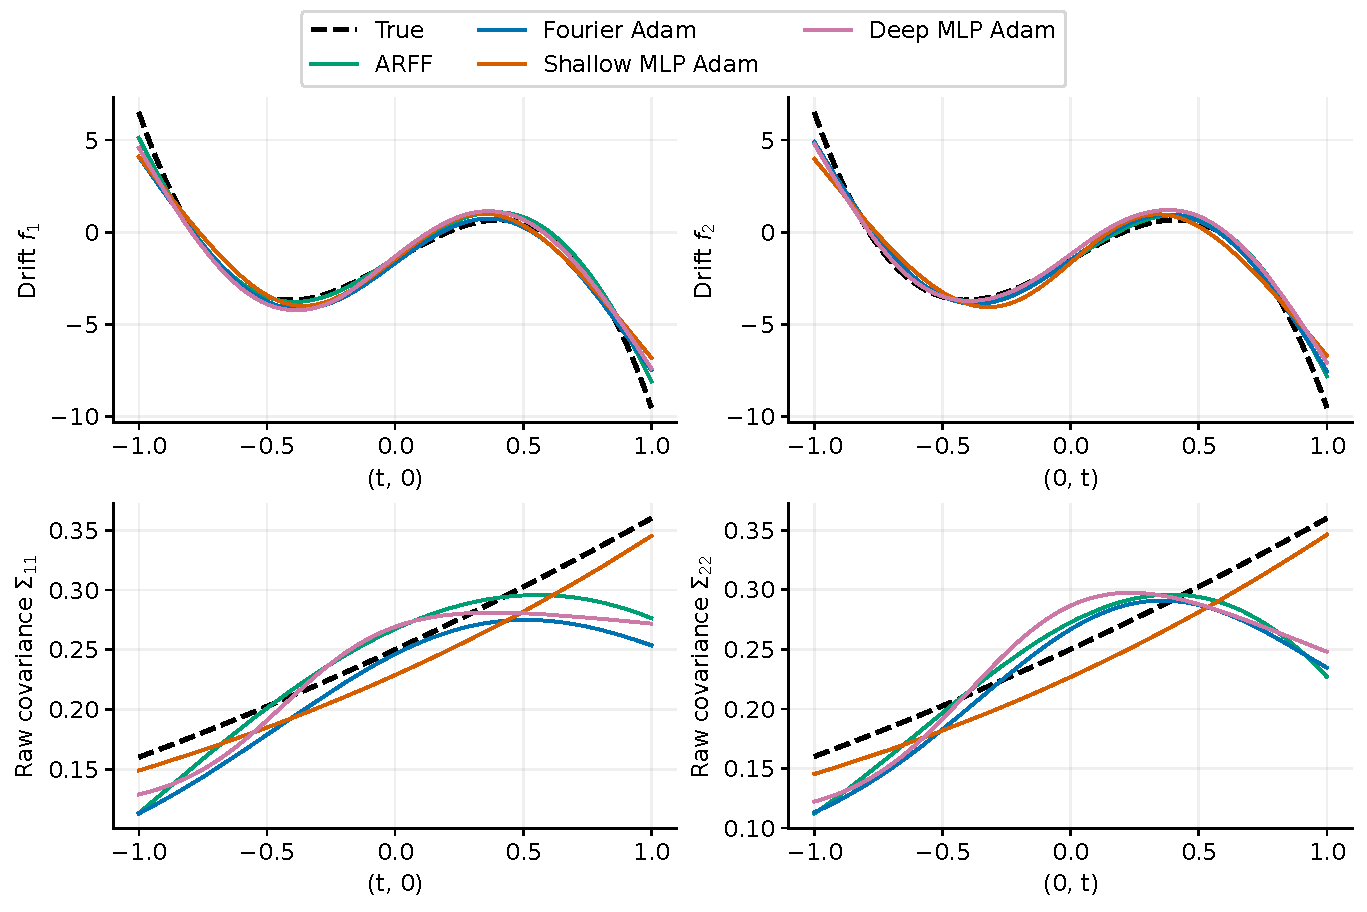
\includegraphics[width=\linewidth]{../figures/ex1_seed0_recovery.pdf}\caption{Experiment 1: true and learned coefficients on prescribed coordinate slices with 201 points in $[-1,1]$. All four already selected seed-0 models are shown. Seed 0 is illustrative, not representative or best. Covariance is raw $\Sigma$, not its factor or projected estimate. The historical evaluation protocol is validation-selected.}\label{fig:ex1coeff}\end{figure}
\FloatBarrier
\subsection{Epidemic, wave-derived and broad-spectrum applications: Experiments 5--7}
\begin{table}[htbp]\centering\small\caption{Experiment 5: fixed-lag SSA, population 1024. Outer-validation mean $\pm$ sample SD over 30 fitting seeds. Raw covariance RMSE.}\label{tab:ex5}\resizebox{\linewidth}{!}{\begin{tabular}{lrrrr}\toprule Method & Parameters & Drift RMSE & Raw covariance RMSE & NLL\\\midrule
ARFF & 3,072 & $0.002631\pm 0.0003076$ & $4.993\times10^{-6}\pm 9.03\times10^{-7}$ & $-11.98\pm 0.03256$\\
Joint Fourier & 3,072 & $0.06746\pm 0.0001462$ & $0.001017\pm 5.659\times10^{-5}$ & $-11.7\pm 0.001035$\\
Shallow MLP & 2,564 & $0.06767\pm 5.873\times10^{-5}$ & $0.001106\pm 9.235\times10^{-6}$ & $-11.7\pm 0.0001884$\\
Deep MLP & 34,308 & $0.04487\pm 0.003344$ & $0.0002867\pm 1.313\times10^{-5}$ & $-11.79\pm 0.006817$\\
\bottomrule\end{tabular}
}\end{table}
\begin{table}[htbp]\centering\small\caption{Experiment 6: corrected wave labels, effective covariance $(g/2)^2$. Outer-validation mean $\pm$ sample SD over 30 fitting seeds. Raw covariance RMSE.}\label{tab:ex6}\resizebox{\linewidth}{!}{\begin{tabular}{lrrrr}\toprule Method & Parameters & Drift RMSE & Raw covariance RMSE & NLL\\\midrule
ARFF & 4,096 & $0.2823\pm 0.03692$ & $1.904\times10^{-5}\pm 3.253\times10^{-6}$ & $-9.415\pm 5.857\times10^{-5}$\\
Joint Fourier & 4,096 & $3.267\pm 0.002594$ & $9.561\times10^{-5}\pm 1.962\times10^{-5}$ & $-9.411\pm 0.0004083$\\
Shallow MLP & 4,098 & $1.315\pm 1.117$ & $0.0001224\pm 0.0001342$ & $-9.409\pm 0.01172$\\
Deep MLP & 133,634 & $3.002\pm 0.823$ & $2.494\times10^{-5}\pm 2.857\times10^{-6}$ & $-9.412\pm 0.0009847$\\
\bottomrule\end{tabular}
}\end{table}
\begin{table}[htbp]\centering\small\caption{Experiment 7: drift with broad spectral support. Outer-validation mean $\pm$ sample SD over 30 fitting seeds. Raw covariance RMSE.}\label{tab:ex7}\resizebox{\linewidth}{!}{\begin{tabular}{lrrrr}\toprule Method & Parameters & Drift RMSE & Raw covariance RMSE & NLL\\\midrule
ARFF & 6,144 & $0.1057\pm 0.007913$ & $0.0001156\pm 1.175\times10^{-5}$ & $-8.686\pm 0.0002846$\\
Joint Fourier & 6,144 & $0.1593\pm 0.00249$ & $0.0001411\pm 2.15\times10^{-6}$ & $-8.686\pm 0.0001772$\\
Shallow MLP & 5,124 & $0.1962\pm 1.788\times10^{-5}$ & $7.844\times10^{-5}\pm 1.253\times10^{-7}$ & $-8.685\pm 2.356\times10^{-6}$\\
Deep MLP & 134,148 & $0.1004\pm 0.01424$ & $0.0001576\pm 5.652\times10^{-5}$ & $-8.687\pm 0.0001154$\\
\bottomrule\end{tabular}
}\end{table}
The SIR coefficients describe a diffusion approximation to a jump process; row-wise validation can share trajectories with fitting. Favorable raw errors and NLL coexist with ARFF raw-SPD violations in 29/30 Ex5 runs. Ex6 uses the corrected labels without changing state trajectories, but poor neural drift recovery remains. Ex7 has competitive ARFF drift recovery, while deep MLP has slightly lower mean drift error and shallow MLP lower covariance error. These applications demonstrate different strengths and limitations, not a universal winner.

\begin{table}[htbp]\centering\small\caption{Raw ARFF covariance validity. Historical rows use outer validation; Ex8 uses independent test. Minimum eigenvalue is the worst across seeds and points; floor is used for NLL only.}\resizebox{\linewidth}{!}{\begin{tabular}{llrrrr}\toprule Data & Method & Seeds affected & Mean rate (\%) & Min. raw eigenvalue & Floor\\\midrule
EX 1 & ARFF & 0/30 & 0 & 0.073099 & $10^{-6}$\\
EX 2 & ARFF & 0/30 & 0 & $2.8564\times10^{-5}$ & $10^{-6}$\\
EX 3 & ARFF & 0/30 & 0 & 0.010213 & $10^{-2}$\\
EX 5 & ARFF & 29/30 & 5.201 & $-6.6074\times10^{-6}$ & $10^{-6}$\\
EX 6 & ARFF & 0/30 & 0 & 0.00052194 & $10^{-6}$\\
EX 7 & ARFF & 0/30 & 0 & 0.0092772 & $10^{-6}$\\
Ex8 test & ARFF & 30/30 & 45.483 & -0.25729 & $10^{-3}$\\
\bottomrule\end{tabular}
}\end{table}

Historical-to-current numerical differences are not all explained. Established changes include OOF covariance targets, operational SPD handling, fixed-lag SSA, Ex6 labels, and Ex8 float64 integration. Metric populations, covariance-factor conventions and unrecovered historical execution chains also differ. These corrections do not prove the cause of every discrepancy, including Ex1/Ex2 drift, Ex3 near-identical poor fits, Ex6 recovery and Ex7 NLL differences. The detailed reconciliation is retained in the reproducibility record.
\FloatBarrier
\subsection{Experiment 8: near-singular diffusion benchmark}
\begin{table}[htbp]\centering\small\caption{Corrected Ex8: independent-test mean $\pm$ sample SD, all 30 fitting seeds. Raw covariance RMSE; ARFF NLL uses floor $10^{-3}$.}\label{tab:ex8}\resizebox{\linewidth}{!}{\begin{tabular}{lrrrr}\toprule Method & Parameters & Drift RMSE & Raw covariance RMSE & NLL\\\midrule
Joint Fourier & 1,792 & $0.4586\pm 0.0554$ & $0.7445\pm 0.1668$ & $-8.346\pm 0.06502$\\
Split Fourier & 1,792 & $0.6371\pm 0.04144$ & $0.6512\pm 0.1064$ & $-8.35\pm 0.06037$\\
ARFF & 1,792 & $0.9665\pm 0.4239$ & $0.1142\pm 0.002306$ & $-8.898\pm 0.07379$\\
Joint MLP & 1,814 & $0.1593\pm 0.04369$ & $0.2896\pm 0.079$ & $-9.958\pm 0.1774$\\
Split MLP & 1,814 & $0.725\pm 0.1365$ & $0.2225\pm 0.06532$ & $-10.13\pm 0.2216$\\
\bottomrule\end{tabular}
}\end{table}

\begin{figure}[htbp]\centering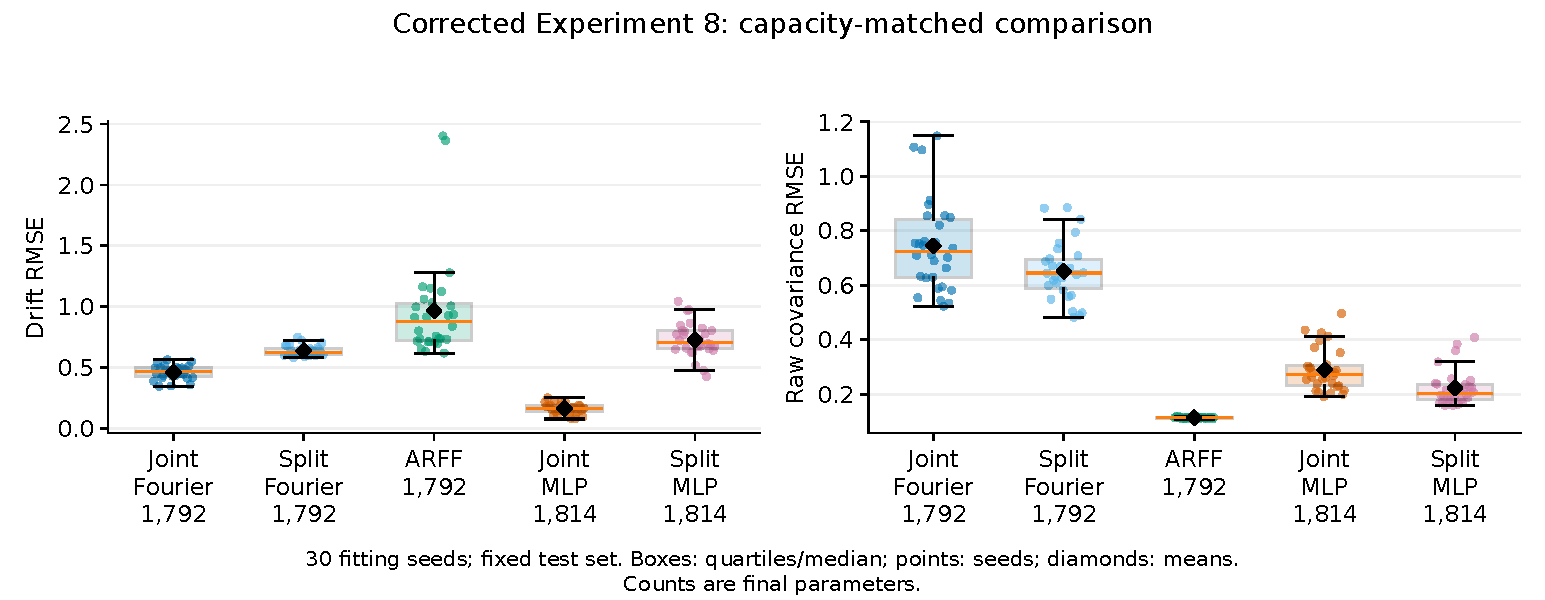
\includegraphics[width=\linewidth]{../figures/baseline.pdf}\caption{Corrected Ex8, all 30 seeds. Boxes show quartiles and median, points individual fitting seeds, diamonds means. Final parameter counts exclude discarded cross-fit models. Covariance error is raw.}\label{fig:ex8distribution}\end{figure}

ARFF has the lowest mean raw covariance error (0.1141) but much poorer drift (0.9665) than Joint MLP (0.1593). Split MLP has lower NLL than ARFF and Joint MLP. Splitting improves mean covariance error for both Adam families but worsens drift in this benchmark. All 30 ARFF models have raw-SPD violations; the mean test rate is 45.48\% and the minimum raw eigenvalue is approximately $-0.2573$. Projection changes the evaluated covariance; low raw coefficient RMSE alone does not guarantee likelihood calibration or validity.

Figures~\ref{fig:ex8drift}--\ref{fig:ex8cov} preserve the original true-versus-learned scientific comparison on corrected models. Their common 100-by-100 cell-centre grid covers $[-2,2]^2$ without the angular singularity at the origin. Each method uses its already selected seed-0 checkpoint, fixed before these evaluations. Shared scales include every method, with no silent clipping. These are deterministic function illustrations, not new stochastic test data; their grid diagnostics do not replace Table~\ref{tab:ex8}.

\begin{figure}[htbp]\centering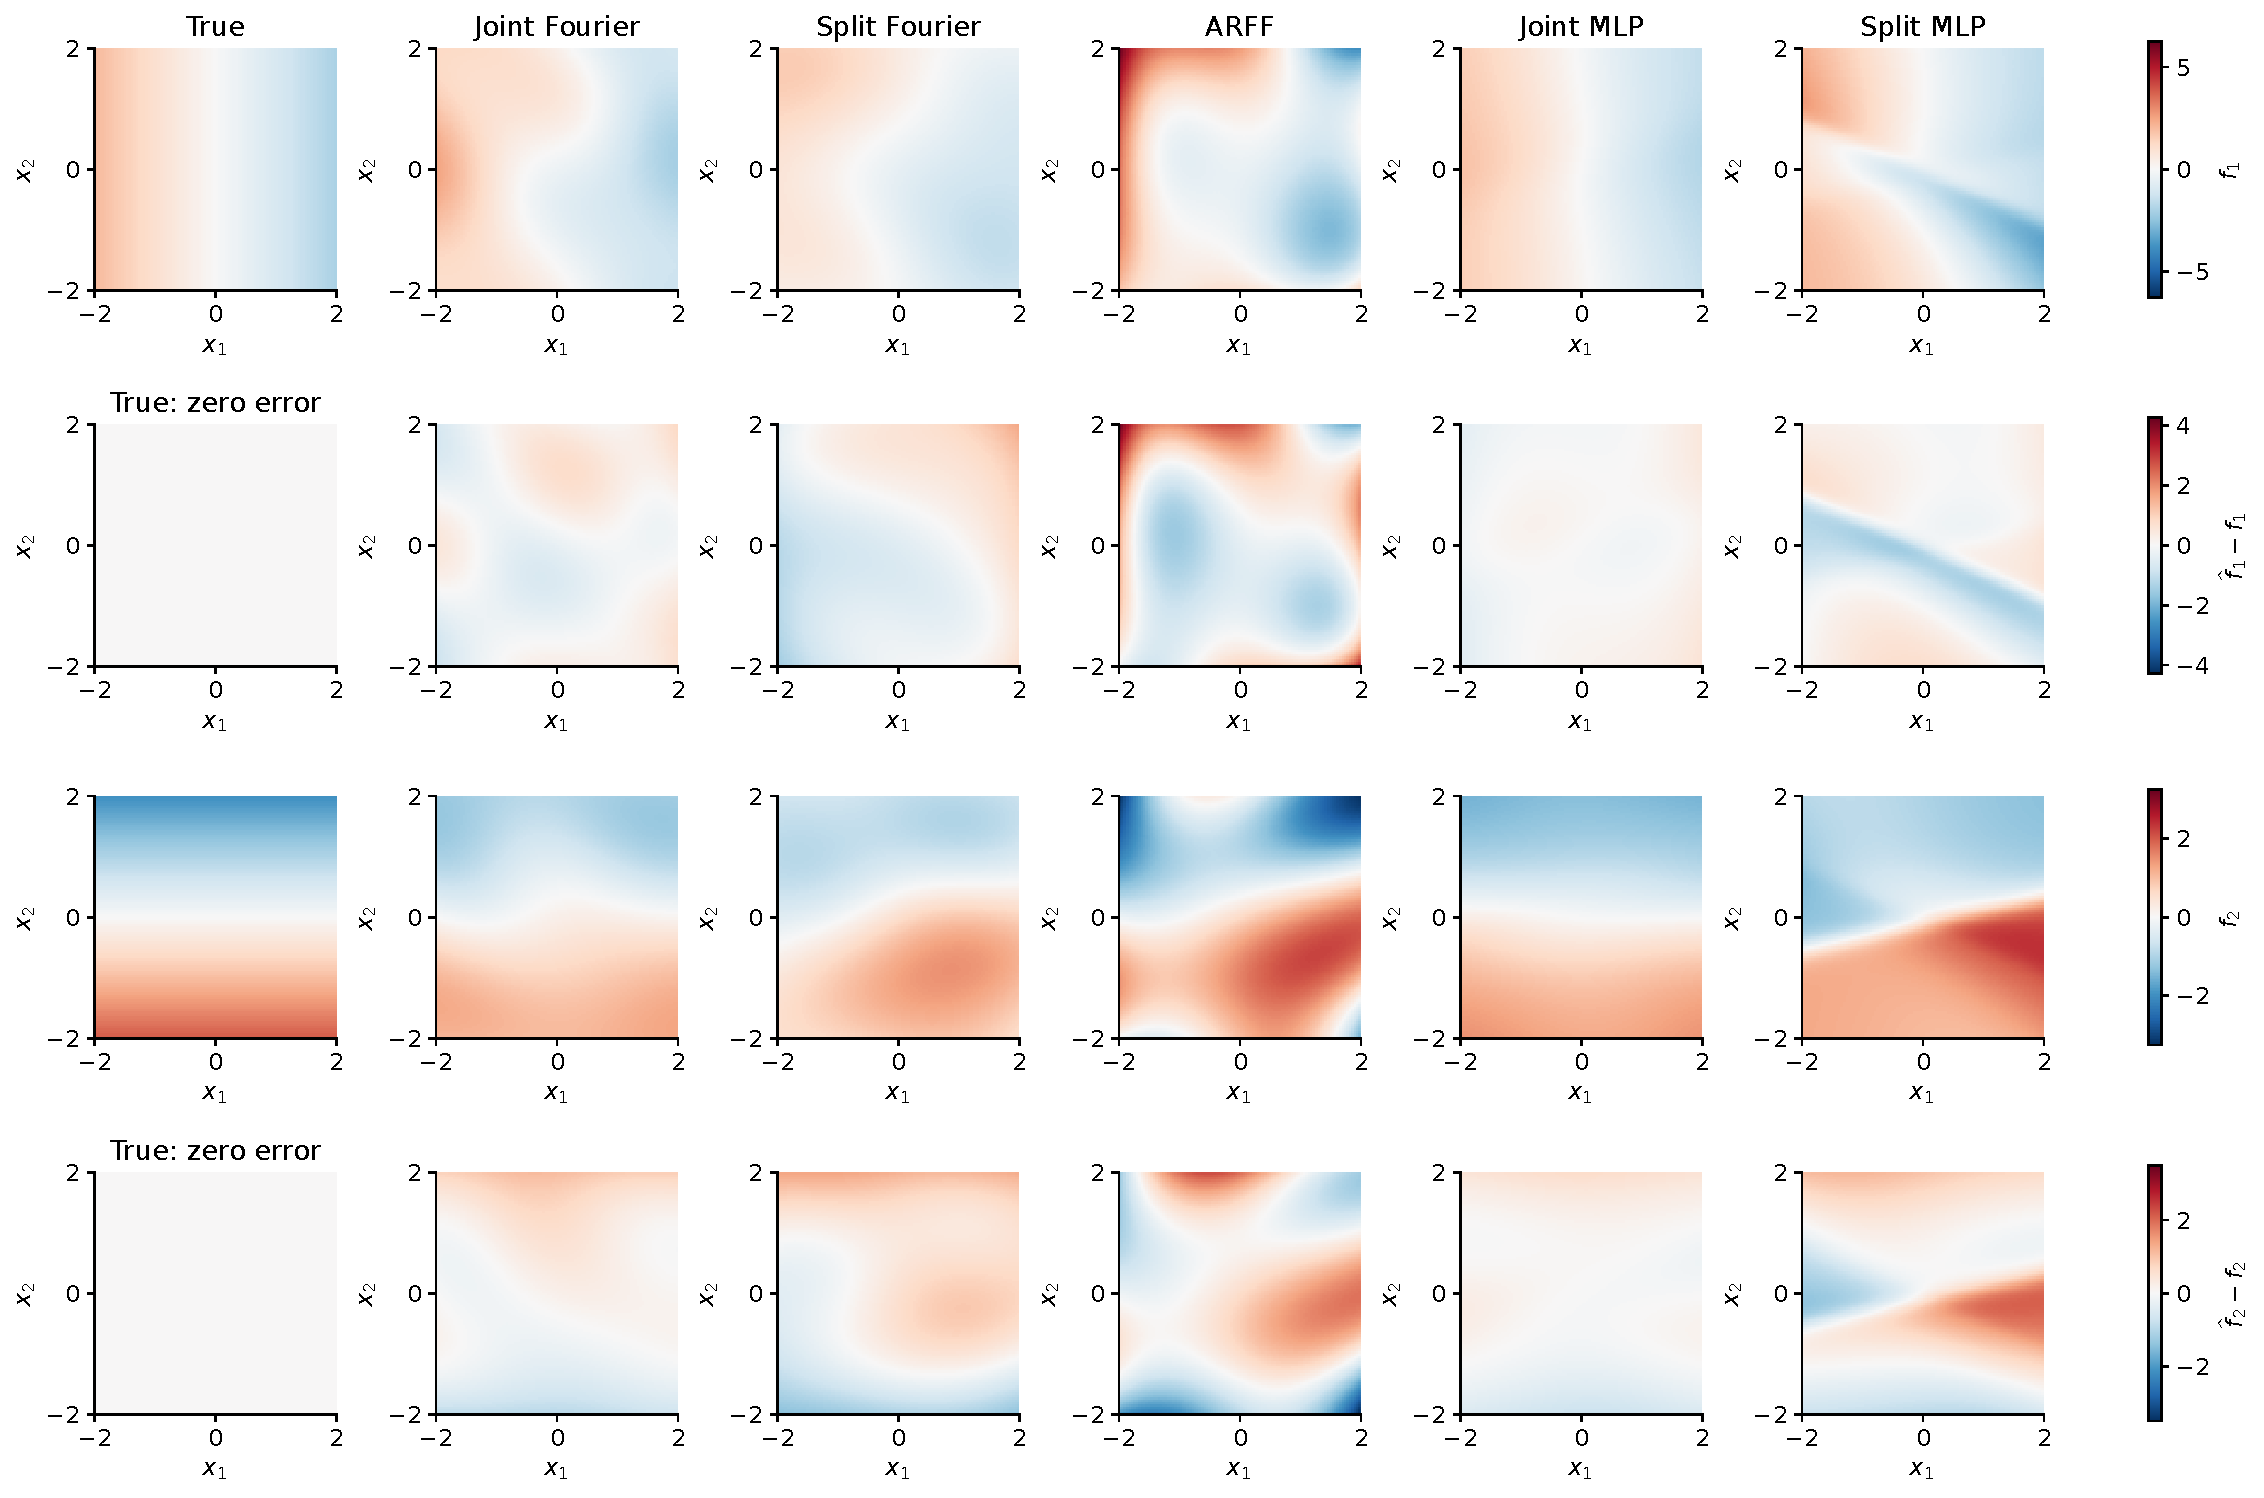
\includegraphics[width=\linewidth]{../figures/ex8_seed0_drift.pdf}\caption{Corrected Ex8 illustrative seed-0 drift. Rows show $f_1$, its signed error, $f_2$, and its signed error; columns are truth and all five estimators. Each row shares a color scale. The true zero-error column is shown explicitly. No checkpoint or seed was chosen from appearance or test performance.}\label{fig:ex8drift}\end{figure}

\begin{figure}[htbp]\centering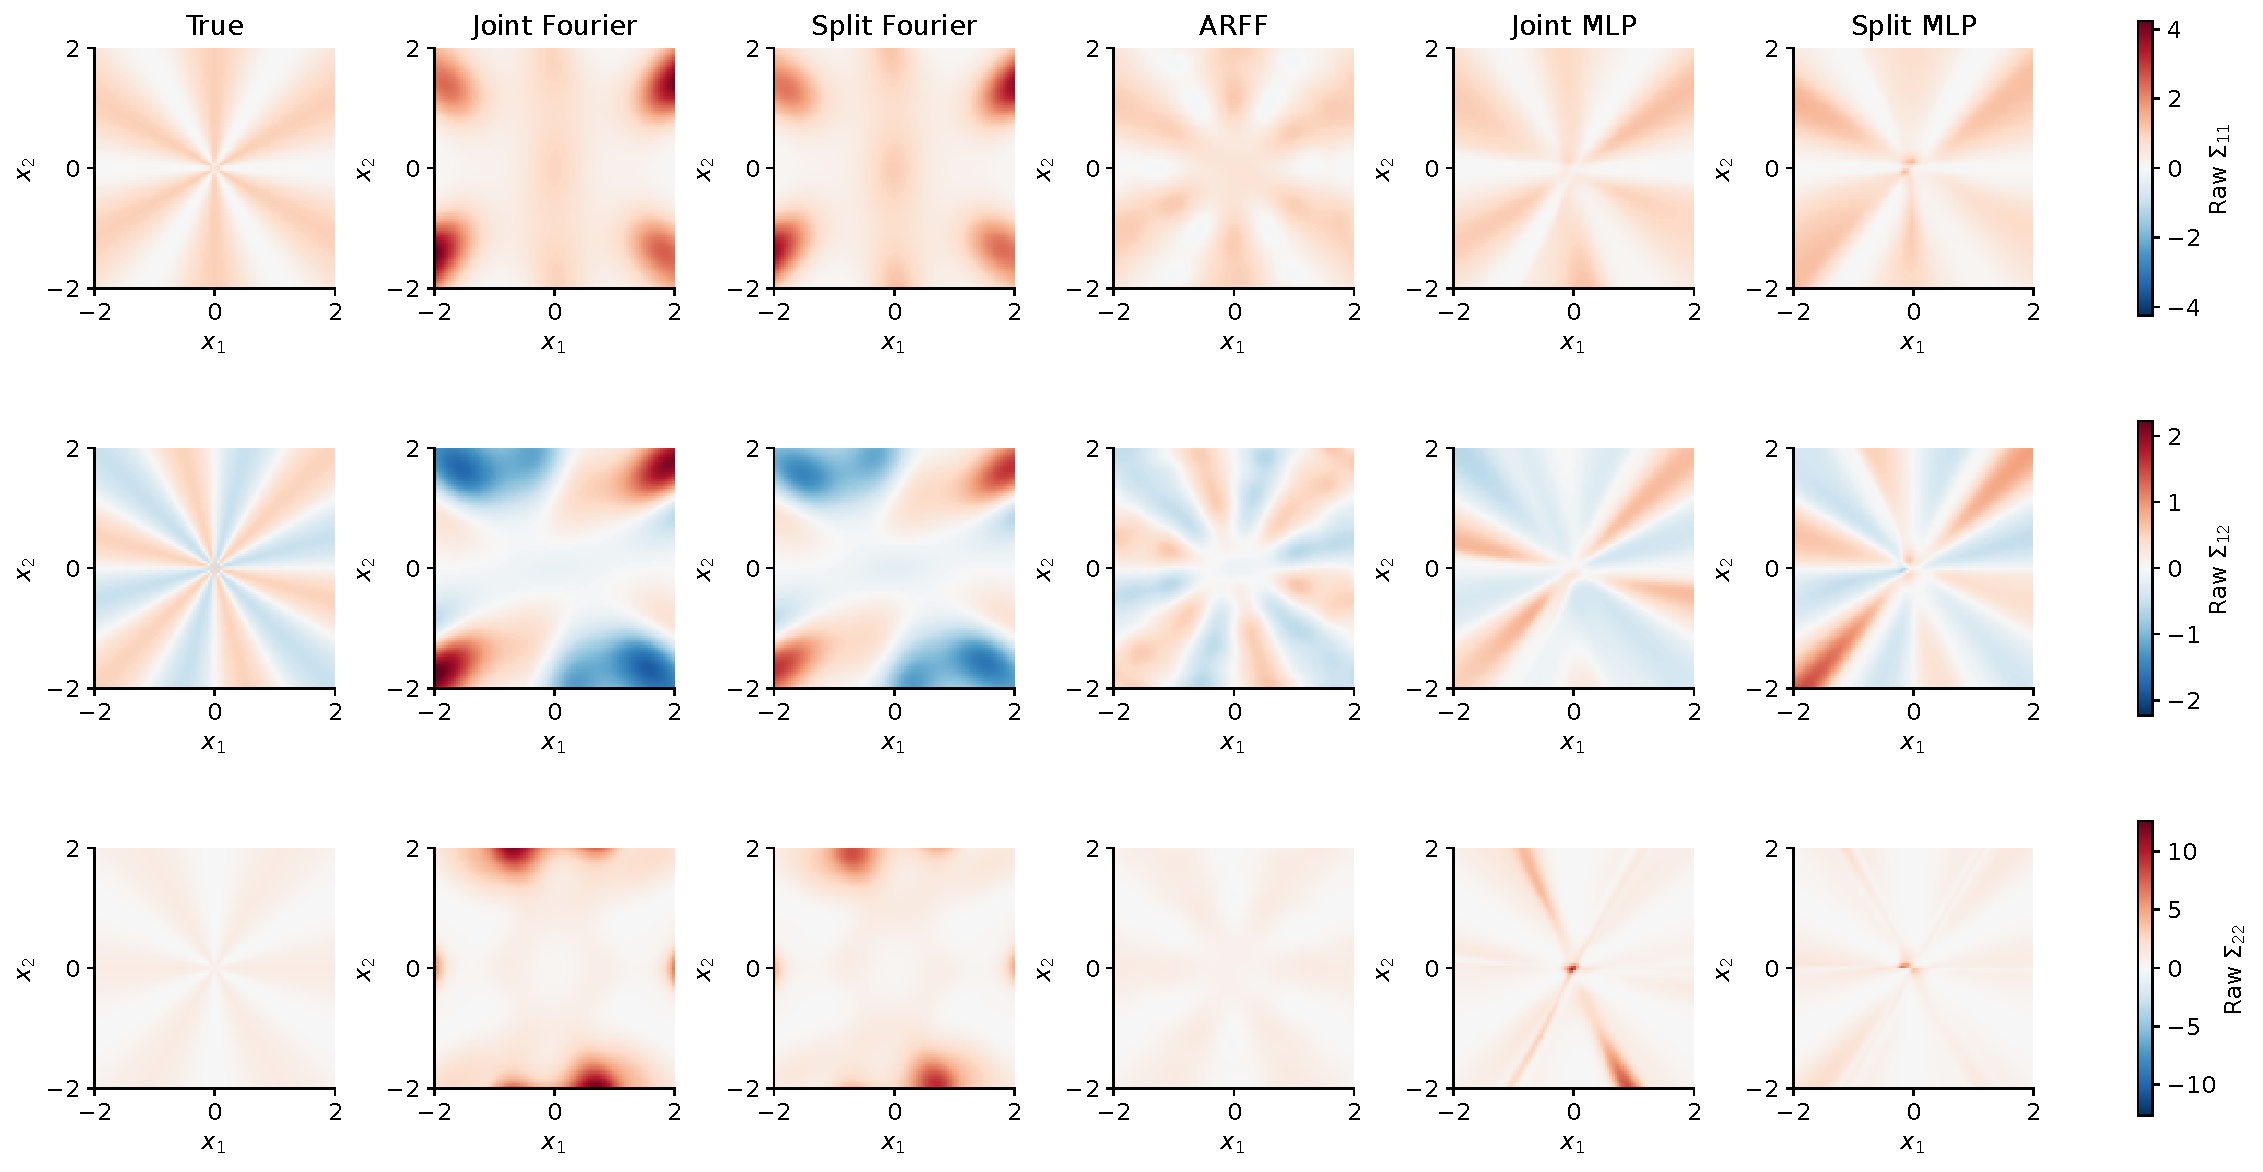
\includegraphics[width=\linewidth]{../figures/ex8_seed0_raw_covariance.pdf}\caption{Corrected Ex8 illustrative seed-0 raw covariance. Rows are $\Sigma_{11},\Sigma_{12},\Sigma_{22}$; columns are truth and all five estimators. Shared scales can make lower-amplitude structure less prominent but do not hide larger errors. These are covariance entries, not diffusion-factor entries. Raw estimates are not projected; the separate projection diagnostic appears in Appendix~\ref{app:projection}.}\label{fig:ex8cov}\end{figure}

\FloatBarrier
\subsection{Empirical Error Analysis}
These completed Ex8 studies replace unsupported historical scaling displays as \emph{different descriptive experiments}. They do not reproduce the historical modified-Ex7 quadratic-covariance or $\mathrm{NLL}_\infty$ procedure, whose execution chain remains incomplete. No rate reference line is fitted. Ten predetermined fitting seeds share nested training data and fixed 10000-point validation/test sets; lag observations are Brownian-coupled.
\subsubsection{Dependence on sample size \texorpdfstring{$N$}{N}}
At $K=1024,h=10^{-4}$, increasing $N$ from 80000 to 640000 lowers ARFF drift RMSE from 0.9297 to 0.4763 and Joint MLP from 0.1389 to 0.06136. The full curves are in Appendix~\ref{app:sensitivity}. Neither a universal rate nor saturation is established.
\subsubsection{Dependence on observation lag \texorpdfstring{$h$}{h}}
All nine lags from $2.5\times10^{-5}$ to .002 are retained. Larger-lag points were admitted only under the prescribed discrete linear-drift relative-bias tolerance $10^{-3}$, not method rankings. ARFF drift continues improving while its raw covariance error remains near .08; split-method drift is non-monotone and Joint MLP relatively insensitive. This criterion bounds drift bias, not covariance finite-lag error.
An exploratory, three-seed ARFF intervention at three of these lags changes only the drift ridge penalty in the five nuisance fits and final drift fit; the covariance penalty stays at .001. Its paired outcomes, including mixed NLL changes, are reported in Appendix~\ref{app:lag_ridge}. The intervention does not replace the ten-seed lag study or its production setting.

\begin{figure}[htbp]\centering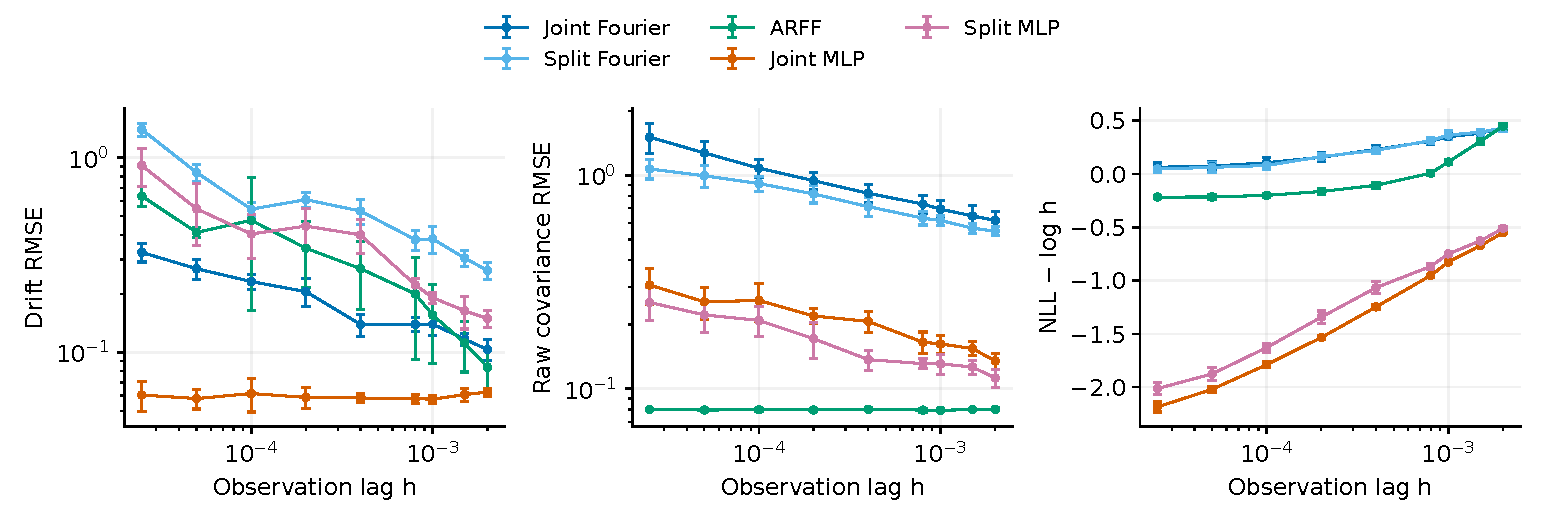
\includegraphics[width=\linewidth]{../figures/h.pdf}\caption{Ex8 test sensitivity to lag at $N=640000,K=1024$, mean $\pm$ sample SD over ten fitting seeds. $\mathrm{NLL}-\log h$ removes the two-dimensional density-scale term, not transition-shape differences. The .002 endpoint satisfies the pre-existing oracle bias tolerance, not a fitted optimum.}\label{fig:hmodern}\end{figure}

\subsubsection{Dependence on feature dimension \texorpdfstring{$K$}{K}}
Phase-1 validation equivalence failed for both sample size and lag; the preregistered fallback $N=640000,h=10^{-4}$ defines this capacity comparison. It is not an established capacity-dominated regime. ARFF raw covariance improves across capacity but drift is non-monotone and changes little between endpoints. Fourier drift deteriorates at larger widths; Joint MLP generally improves before a small high-width reversal, whereas Split MLP drift worsens across these points. These outcomes do not support an empirical $O(1/K)$ claim.

\begin{figure}[htbp]\centering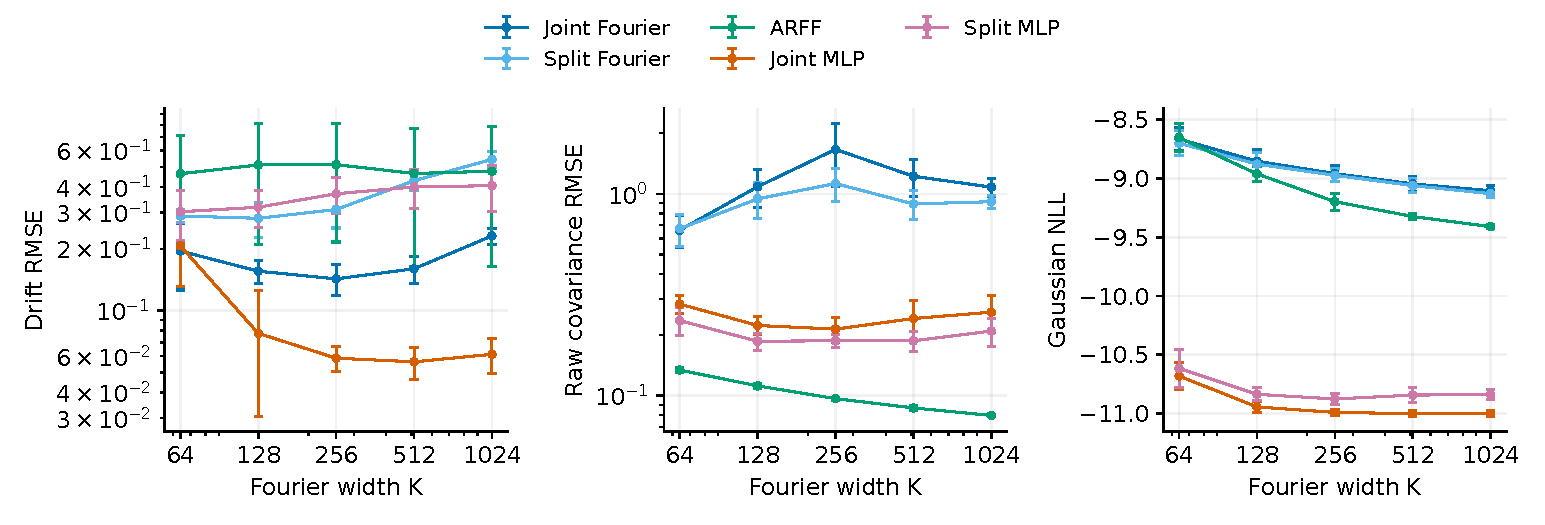
\includegraphics[width=\linewidth]{../figures/capacity.pdf}\caption{Descriptive Ex8 test performance versus Fourier width $K$ at fixed $N=640000,h=10^{-4}$, ten seeds. Error bars show one sample SD about the fitting-seed mean, not a confidence band. $K=64,128,256,512,1024$ gives Fourier parameter counts 896,1792,3584,7168,14336; matched two-layer MLP widths 18,27,39,57,81 give counts 887,1814,3554,7244,14180. No asymptotic rate is asserted.}\label{fig:kmodern}\end{figure}

\section{Summary and Discussion}\label{sec:summary}
This work develops a conditional-moment motivated two-stage ARFF procedure for SDE coefficient learning. Its practical appeal is the explicit separation of drift and covariance targets and linear multi-output amplitude solves for fixed frequencies. The polynomial, epidemic, wave-derived and spectrally broad applications demonstrate its scope while retaining historical protocol differences. The corrected independent-test near-singular comparison shows strong raw covariance recovery but poorer drift than Joint MLP and inferior NLL to neural alternatives. There is no single ranking across these quantities.

Five-fold cross-fitting is implemented, not future work. It excludes each observation from its own nuisance fit and selection but does not remove drift error, finite-lag bias or dependent-data issues. Raw covariance may be indefinite; projection is explicit and distinct from coefficient recovery. Descriptive N/h/K evidence does not establish rate bounds or capacity dominance.

Separate shared-noise surrogate studies illuminate fixed-basis variance, ridge shrinkage and mixed selected-checkpoint resampling outcomes (Appendix~\ref{app:drift_diagnostic}). They neither establish a unique mechanism nor change the production ridge. Hybrid component and floor diagnostics also distinguish covariance recovery from likelihood calibration; the instantaneous-coefficient oracle is not the true finite-lag likelihood optimum.

Extending transition approximations or assessing longer-time dynamics remains scientifically interesting, but the current evidence concerns coefficient recovery and Gaussian scoring. We make no trajectory-fidelity or isolated-runtime superiority claim. Ex4's unresolved convention is retained as an author-review issue rather than silently repaired. Public-release details and unresolved historical execution differences are documented separately.

\bibliographystyle{plain}
\bibliography{references}

% ============================================================
%  Appendices: former supplementary materials integrated below
% ============================================================
\appendix

% ============================================================
%  APPENDIX B — Experiment Details
% ============================================================
\section{Details for Numerical Experiments}
\label{app:num_experiments}

This appendix preserves the application data specifications. Ex4 is a historical specification with an unresolved sign/conditioning convention, not an endorsed numerical comparison. Corrected data versions and effective splits are stated explicitly.

\subsection{Experiments 1--4 and 7--8: SDE snapshot generation}

For Experiments 1--3 and 7--8, stored snapshots use fine EM simulation; Ex4 remains withheld. Each sample begins from an initial condition $x_0$ drawn uniformly from a specified domain $\mathcal{D}_{x_0}$. From this initial state, the SDE is evolved for 1000 EM iterations with internal step size $\Delta t = h/1000$, corresponding to a total transition time $h$. Only the initial and final states are retained, yielding training triples $(x_0, x_1, h)$.

Ex8 baseline integration and endpoint differences use float64, with unchanged initial states, normal draws and 80/10/10 split IDs. Estimator arithmetic is float32. Historical Ex1--3,5--7 use 90/10 train/validation obtained from the canonical permutation; their validation results are selected-validation evidence. Lag extensions keep the fine step $10^{-7}$ and change substep count, rather than fixing 1000 substeps for every lag.

Training data parameters are summarized in Tables \ref{tab:polynomial_training_data}-\ref{tab:near_singular_data}.

\begin{table}[H]
\centering
\small
\caption{Summary of the training data for the polynomial experiments 1--3.}
\label{tab:polynomial_training_data}
\begin{tabular}{@{}c c c c c c c@{}}
\toprule
Exp. & Dim. & True Drift $f(x)$ & True Diffusion $\sigma(x)$ & Step $h$ & $\mathcal{D}_{x_0}$ & \#Pts \\
\midrule
1 & 2 &
\footnotesize $\begin{bmatrix} -16x_0^{3} + 8x_0 - 1.5 \\ -16x_1^{3} + 8x_1 - 1.5 \end{bmatrix}$ &
\footnotesize $\begin{bmatrix} 0.1x_0 + 0.5 & 0 \\ 0 & 0.1x_1 + 0.5 \end{bmatrix}$ &
0.01 & $[-1,1]^2$ & 10000 \\

2 & 3 &
\footnotesize $\begin{bmatrix} -x_0 \\ -x_1 \\ -x_2 \end{bmatrix}$ &
\footnotesize $\begin{bmatrix} 0.09506 & 0 & 0 \\ 0.04639 & 0.15817 & 0 \\ 0.04338 & 0.07507 & 0.00853 \end{bmatrix}$ &
0.01 & $[-1,1]^3$ & 10000 \\

3 & 10 &
\begin{tabular}[c]{@{}c@{}}
$f(x) = (g(x_0), \ldots, g(x_9))^{\top}$ \\
$g(t) = -16t^{3} + 8t - 1.5$
\end{tabular} &
see below &
0.01 & $[-1,1]^{10}$ & 100000 \\
\bottomrule
\end{tabular}
\end{table}

True diffusion for Experiment 3
{\scriptsize
\begin{equation*}
\begin{aligned}
&\sigma(x) =\\
&\begin{bmatrix}
  0.22832 & 0.010865 & 0.090003 & -0.060878 & 0.012992 & -0.009347 & -0.029005 & 0.054890 & -0.095809 & -0.007837 \\[2pt]
  0.010865 & 0.13756 & 0.003815 & 0.012116 & -0.003058 & 0.014402 & 0.005206 & 0.007598 & 0.049540 & -0.024421 \\[2pt]
  0.090003 & 0.003815 & 0.27686 & -0.073250 & -0.057378 & 0.077955 & -0.067661 & 0.011554 & -0.123940 & 0.032760 \\[2pt]
 -0.060878 & 0.012116 & -0.073250 & 0.27916 & 0.020965 & 0.017321 & 0.054022 & -0.077201 & 0.072615 & -0.063557 \\[2pt]
  0.012992 & -0.003058 & -0.057378 & 0.020965 & 0.22742 & -0.057193 & 0.003315 & -0.013105 & 0.022512 & -0.009778 \\[2pt]
 -0.009347 & 0.014402 & 0.077955 & 0.017321 & -0.057193 & 0.21696 & -0.023792 & -0.003358 & -0.011393 & -0.012749 \\[2pt]
 -0.029005 & 0.005206 & -0.067661 & 0.054022 & 0.003315 & -0.023792 & 0.14159 & -0.004788 & 0.053163 & -0.029238 \\[2pt]
  0.054890 & 0.007598 & 0.011554 & -0.077201 & -0.013105 & -0.003358 & -0.004788 & 0.20365 & -0.021602 & 0.008506 \\[2pt]
 -0.095809 & 0.049540 & -0.123940 & 0.072615 & 0.022512 & -0.011393 & 0.053163 & -0.021602 & 0.29429 & -0.043131 \\[2pt]
 -0.007837 & -0.024421 & 0.032760 & -0.063557 & -0.009778 & -0.012749 & -0.029238 & 0.008506 & -0.043131 & 0.19488
\end{bmatrix}.
\end{aligned}
\end{equation*}}

\begin{table}[H]
\centering
\small
\caption{Historical underdamped Langevin specification, retained for author review only: drift sign and conditioning unresolved; numerical comparison withheld.}
\label{tab:Langevin_training_data}
\begin{tabular}{@{}c c c c c c c c c@{}}
\toprule
Exp. & $v_0$ Dim. & $x_0$ Dim. & \begin{tabular}[c]{@{}c@{}}True Drift\\ $f(x, v)$\end{tabular} &
\begin{tabular}[c]{@{}c@{}}True Diffusion\\ $\sigma(x, v)$\end{tabular} & Step $h$ & $\mathcal{D}_{v_0}$ & $\mathcal{D}_{x_0}$ & \#Pts \\
\midrule
4 & 1 & 1 & $-x^3 - x + 0.5v$ & $\sqrt{0.1}$ & 0.01 & $[-1,1]$ & $[-1,1]$ & 10000 \\
\bottomrule
\end{tabular}
\end{table}

\begin{table}[H]
\centering
\small
\caption{Summary of the training data for the wide spectral support experiment.}
\label{tab:wide_spectrum_data}
\begin{tabular}{@{}c c c c c c c@{}}
\toprule
Exp. & Dim. & True Drift $f(x)$ & True Diffusion $\sigma(x)$ & Step $h$ & $\mathcal{D}_x$ & \#Pts \\
\midrule
7 & 2 &
\footnotesize $\begin{bmatrix}
e^{-|x_0|/0.1} e^{-\frac{1}{2}(x_0^2 + x_1^2)} \\
e^{-|x_1|/0.2} e^{-\frac{1}{2}(x_0^2 + x_1^2)}
\end{bmatrix}$ &
\footnotesize $\begin{bmatrix} 0.1 & 0 \\ 0 & 0.1 \end{bmatrix}$ &
0.001 & $[-1,1]^2$ & 100000 \\
\bottomrule
\end{tabular}
\end{table}

The historical modified-Ex7 error-analysis specification, whose execution/NLL-infinity chain is not authenticated here, used diffusion $\sigma(x)$ = $\begin{bmatrix} 0.25x_0^2 + 0.25 & 0 \\ 0 & 0.25x_1^2 + 0.25 \end{bmatrix}$.


\begin{table}[H]
\centering
\small
\caption{Summary of the training data for the near singular diffusion experiment.}
\label{tab:near_singular_data}
\begin{tabular}{@{}c c c c c c c@{}}
\toprule
Exp. & Dim. & True Drift $f(x)$ & True Diffusion $\sigma(x)$ & Step $h$ & $\mathcal{D}_x$ & \#Pts \\
\midrule
8 & 2 &
\footnotesize $\begin{bmatrix}-x_0\\-x_1\end{bmatrix}$ &
\footnotesize
\begin{tabular}{@{}c@{}}
$R(\vartheta(x))
\begin{bmatrix}
0.0001 & 0\\
0 & 1
\end{bmatrix}
R(\vartheta(x))^\top$ \\[4pt]
{\scriptsize $R(\vartheta)$: planar rotation matrix} \\[2pt]
{\scriptsize $\vartheta(x)=3\,\mathrm{atan2}(x_1,x_0)$}
\end{tabular}
&
0.0001 & $[-2,2]^2$ & 100000 \\
\bottomrule
\end{tabular}
\end{table}


\subsection{Experiment 5: SIR data generation}

Data for Experiment~5 are generated using Gillespie's stochastic simulation algorithm (SSA) applied to the SIRS jump process described in Section~\ref{sec:computational_experiments}. The system tracks integer-valued populations $(n_0,n_1,n_2)$ corresponding to susceptible, infected, and recovered individuals, with concentrations $\tilde{x}_p = n_p/N$.

The concentration-level rates are $r_1 = 4k_1\tilde{x}_0\tilde{x}_1,
r_2 = k_2\tilde{x}_1,
r_3 = k_3\tilde{x}_2,$ and count-process hazards are $Nr_1,Nr_2,Nr_3$, with $N=1024$. An event is selected proportionally. The holding time is sampled as $\Delta \tau = -\log(U_1)/(N(r_1+r_2+r_3))$, where $ U_1\sim\mathrm{Uniform}(0,1)$.

Training data are generated from multiple independent trajectories. Initial concentrations $(\tilde{x}_0,\tilde{x}_1,\tilde{x}_2)$ are sampled uniformly from the two-simplex subject to the constraint that $N\tilde{x}_p$ is integer-valued. \textcolor{black}{Each trajectory is followed to time 4 with absorbing states handled by the documented absorbing-start exclusion.}

Trajectory observations are the piecewise-constant SSA states at prescribed times separated by $\Delta t=.01$, not the first event after each time. Consecutive observations form fixed-lag triples in susceptible/recovered fractions. There are 99719 retained rows from 250 trajectories. Row-wise splitting can share trajectories and therefore is not independent-trajectory generalization. The infected proportion $\tilde{x}_1$ is omitted since $\tilde{x}_0+\tilde{x}_1+\tilde{x}_2=1$.

Training data was generated according to Table~\ref{tab:SIR_training_data}.
\begin{table}[H]
\centering
\small
\caption{Summary of the training data for the SIR experiment.}
\label{tab:SIR_training_data}
\begin{tabular}{@{}c c c c c c c@{}}
\toprule
Exp. & $N$ & Parameters $k$ & Max Time (s)& No. Traj. & Sample Step Size $\Delta t$ (s)& Retained \#Pts \\
\midrule
5 & 1024 & $k_1,k_2,k_3 = 1,1,0$ & 4 & 250 & 0.01& 99719\\
\bottomrule
\end{tabular}
\end{table}

\subsection{Experiment 6: Stochastic wave equation data generation}

Training data for Experiment 6 are generated by numerically solving the stochastic wave equation described in Section \ref{sec:computational_experiments} on a uniform space-time grid using the staggered-grid scheme in (\ref{eq:wave_scheme}). The grid spacing $h$ defines the staggered spatial/time construction rather than the effective regression lag, and defines the temporal discretization $t_j = jh$ and the spatial discretization $x_i = ih$, and therefore controls the resolution of the numerical solution and the resulting number of training samples. The computed solution is converted using the corrected exact stencil identity, with effective lag $h^2/4$ at initialization and $h^2/2$ thereafter, independent driving normal variances $h^2$ and $2h^2$, and regression factor $g/2$ rather than $g$. The original states/increments are unchanged by the correction of 498 initial lags and 497502 alternating-grid coordinates. The retained data version is \texttt{ex6\_labels\_v2.npz}. The reformulation is described in Section \ref{sec:computational_experiments}. Ex8 baseline integration and endpoint differences use float64, with unchanged initial states, normal draws and 80/10/10 split IDs. Estimator arithmetic is float32. Historical Ex1--3,5--7 use 90/10 train/validation obtained from the canonical permutation; their validation results are selected-validation evidence. Lag extensions keep the fine step $10^{-7}$ and change substep count, rather than fixing 1000 substeps for every lag.

Training data parameters are summarized in Table \ref{tab:SPDE_training_data}.

\begin{table}[H]
\centering
\small
\caption{Summary of the training data for the stochastic wave equation experiment.}
\label{tab:SPDE_training_data}
\begin{tabular}{@{}c c c c c c c c c c@{}}
\toprule
Exp. & Dim. & $f(x,t,u)$ & $g(x)$ (forcing amplitude) & $u_0(x)$ & $v_0(x)$ & Step $h$ & $\mathcal{D}_x$ & $\mathcal{D}_t$ & Mean \#Pts \\
\midrule
6 & 1 &
\footnotesize $5\sin(4\pi x)$ &
\footnotesize $\frac{1}{20}\left(1+e^{-150(x-\frac12)^2}\right)$ &
\footnotesize $\frac{1}{20} e^{-150(x-\frac12)^2}$ &
\footnotesize $-2 \frac{du_0}{dx}$ &
0.001 & $[0,1]$ & $[0,2]$ & 995004 \\
\bottomrule
\end{tabular}
\end{table}


The Experiment 3 matrix above is displayed to the original decimal precision; exact entries used for evaluation are retained in the accompanying source snapshot of \texttt{src/experiments/definitions.py}.


% ============================================================
%  APPENDIX C — Reproducibility
% ============================================================
\section{Reproducibility and Implementation Details}
\label{app:reproducibility}




\subsection{Fixed training settings}



\begin{table}[H]
\caption{Historical-compatible ARFF settings for retained applications, and modern Ex8 settings. All use $\gamma=1$ and five-fold cross-fitting; inner loop variants are distinguished in the text.}
\label{tab:hyperparams}
\centering
\begin{tabular}{cccccccc}
\hline
Experiment & $\log_2(K)$ & $\delta$ & $\lambda$ & $M_{\min}$ & $M_{\max}$ & Resampling & Metropolis \\ \hline
1 & 8 & 0.05 & 1.00E-03 & 30 & 1000 & True & False \\
2 & 7 & 0.01 & 1.00E-05 & 20 & 1000 & True & False \\
3 & 10 & 0.01 & 1.00E-02 & 50 & 1000 & True & False \\

5 & 8 & 0.1  & 2.00E-03 & 20 & 1000 & True & False \\
6 & 9 & 0.3  & 1.00E-03 & 50 & 1000 & True & False \\
7 & 9 & 0.5  & 1.00E-02 & 50 & 1000 & False & True \\
8 & 7 & 0.2 & 1.00E-03 & 300 & 300 & False & True \\ \hline
% 1 (CPU) & 8 & 0.5 & 1.00E-02 & 30 & 1000 & True & False \\
% 2 (CPU) & 7 & 0.1 & 1.00E-03 & 20 & 1000 & True & False \\ \hline
\end{tabular}
\end{table}

\begin{table}[H]
\caption{Adam hyperparameters.
Historical deep = two hidden layers of width $K/2$; Ex8 both MLPs = two layers of width 27. Historical column is $\log_2 K$; Ex8 MLP row explicitly gives width.}
\label{tab:adam_hyperparams}
\centering
\begin{tabular}{ccccc}
\hline
Experiment & $\log_2(K)$ & $\log_2($Batch Size$)$ & Learning Rate & Epochs \\ \hline
1 & 8  & 9  & 1.00E-03 & 800 \\
2 & 7  & 8  & 1.00E-04 & 100 \\
3 & 10 & 10 & 1.00E-04 & 300 \\

5 & 8  & 8  & 1.00E-04 & 100 \\
6 & 9  & 9  & 1.00E-03 & 600 \\
7 & 9 & 9 & 1.00E-04 & 300 \\
8 Fourier & 7 & 8 & 1.00E-04 & 300 \\
8 MLP & \multicolumn{1}{c}{width 27} & 8 & 1.00E-03 & 300 \\ \hline
% 1 (CPU) & 8 & 6 & 1.00E-03 & 200 \\
% 2 (CPU) & 7 & 6 & 1.00E-03 & 200 \\ \hline
\end{tabular}
\end{table}



\subsection{Selection, information and covariance conventions}
Historical ARFF uses resampling before mutation when enabled, a key-based internal 10\% holdout, earliest strict-minimum ties and zero-based adaptation indexing. The five-point float32 moving sum and historical stopping check precede retention of the terminal candidate. There is no full-data refit. Ex8 instead uses Algorithm~\ref{alg:ARFF}, 300 fixed adaptations, no resampling and one-based post-adaptation selection. In all applications the auxiliary drift fits construct OOF targets.

Historical Adam keeps the legacy initializer and epoch-indexed shuffling keys, retaining the earliest outer-validation NLL minimum without refitting. Shallow tanh has width $K$, deep has two layers of width $K/2$. For Ex3 the historical symmetric diffusion factor is $LL^\top$, so covariance is $(LL^\top)^2$; this is not the modern Ex8 covariance $LL^\top$. Historical diagonal covariance uses softplus outputs. Coefficient comparisons always use $\Sigma=\sigma\sigma^\top$.

Ex8 joint and split Fourier models have 1792 retained parameters each; two-layer width-27 MLP models have 1814. Fourier amplitudes initialize as $.01$ times standard normals and frequencies as standard normals for Adam. MLP uses Glorot-uniform weights, zero biases and covariance final-layer weight scaling $.01$. Full covariance factor diagonals use softplus plus $10^{-8}$. Adam moments are $(.9,.999)$ and epsilon $10^{-7}$. Joint checkpoints minimize external-validation NLL; split drift minimizes validation MSE and split covariance validation NLL. Joint/split pairs share initialization family, not identical key consumption across seven fits versus one.

Outer Ex8 training has 80000 observations; ARFF final amplitudes use 72000 and each OOF nuisance amplitude fit 57600. Adam final models use 80000 and each nuisance model 64000. Historical 90/10 splits use the canonical permutation, with all recorded rows retained. Final parameter counts exclude auxiliary models; two-stage timing includes their fits.

\subsection{System, timing and reproducibility}
Accuracy campaigns ran concurrently across four NVIDIA RTX A6000 GPUs. Per-artifact source/data hashes and environment metadata identify each execution; no single stale package-version table is substituted for these records. Compilation/warm-up, algorithm time, final metric evaluation and serialization are separate scopes. Non-isolated algorithm times are not a publication-quality speed comparison. No new timing run was used for this revision.

\subsection{Coefficient-figure reconstruction}
All new coefficient figures use already selected seed-0 checkpoints, declared illustrative before evaluation. Reconstruction on the original Ex1 validation and Ex8 test populations passed archived drift RMSE, raw covariance RMSE and NLL checks with $\mathrm{rtol}=10^{-5}$ and $\mathrm{atol}=10^{-6}$ on the original GPU backend. No tolerances or checkpoints changed after evaluation. Ex1 uses 201 points on each coordinate slice through zero; Ex8 uses 100-by-100 cell centres on $[-2,2]^2$, excluding the angular singularity at zero. Coordinates, predictions and source hashes accompany the figures. Their diagnostics do not replace the 30-seed archived metrics.

\subsection{Preprocessing, linear algebra and reproducibility record}
Inputs remain in their physical coordinates: no empirical centering, standardization or whitening is applied in either the historical-compatible or modern protocols. Drift targets are increments divided by their observation lags. ARFF covariance targets are residual outer products divided by lag, stored as diagonal or lower-triangular entries. These are the defining moment transformations, not fitted normalization statistics; no denormalization precedes covariance reconstruction or projection. Adam evaluates residual likelihood in the same physical units. SIR concentrations and the wave-stencil reformulation are observation definitions described in Appendix~\ref{app:num_experiments}, not learned preprocessing.

Amplitude fitting forms the unnormalized real sine/cosine feature matrix, the dense Gram matrix and right-hand side, with JAX \texttt{Precision.HIGHEST} matrix products in float32. It solves $(\Phi^\top\Phi+n\lambda I)B=\Phi^\top Y$ through \texttt{jnp.linalg.solve}, the general dense LU solve, not an iterative method or a specified Cholesky solve. There is no iterative tolerance. Features are materialized and recomputed for each amplitude solve and prediction at the requested frequencies, not cached across adaptation. Dataset integration precision is a separate choice.

For the historical-compatible implementation, resampling probabilities are proportional to the pooled sine/cosine/output amplitude norm guarded below by dtype tiny; $K$ draws with replacement precede mutation. The optional Metropolis ratio guards the old norm only, unlike the two-norm guard in modern Algorithm~\ref{alg:ARFF}. For zero-based iteration $i$, the float32 moving average uses the latest $\min(i+1,5)$ validation errors. If its earliest strict-minimum index is $j$, stopping occurs when $j+5<i$ and $i>M_{\min}$; the stopping candidate is excluded from retained-model selection. These are corrected historical-compatible rules, not a claim that every original execution is authenticated.

The baseline and retained application seed lists are $0,\ldots,29$; descriptive Ex8 $N/h/K$ studies use $0,\ldots,9$; lag--ridge uses $0,1,2$. Exact arm manifests and source hashes accompany the archived evidence. Historical tuning ranges, trial budgets and complete execution chains are not fully recoverable. Fixed settings and matched final parameter counts do not establish equal tuning budgets.

Code and the review evidence package are available at \url{https://github.com/ojldoug/SDE_ARFF_2026}, branch \texttt{aku/reproducible-pipeline}. The reproduction-package base is commit \texttt{a8809cd}; subsequent review corrections are identified by repository history. Root \texttt{REPRODUCING.md} maps every table and figure to inputs and commands; \texttt{requirements-dev.txt} records the environment. Compact aggregates and validated coefficient grids permit an archive-only CPU rebuild. Large datasets, checkpoints and complete execution archives are not distributed in ordinary Git and have no durable public download identifier yet. The isolated-checkout build was tested with the existing environment, not a fresh dependency installation. It verifies tables/figures/PDFs, not a fresh training reproduction.

\section{Raw covariance and projection in Experiment 8}\label{app:projection}
The raw covariance map and the matrix used in NLL are distinct. This illustrative seed-0 diagnostic uses the same prescribed grid as the main coefficient figures. Projection is the existing symmetrization/eigenvalue floor at $10^{-3}$, whereas the smallest true instantaneous eigenvalue is $10^{-8}$. No floor was tuned for the plot.
\begin{figure}[htbp]\centering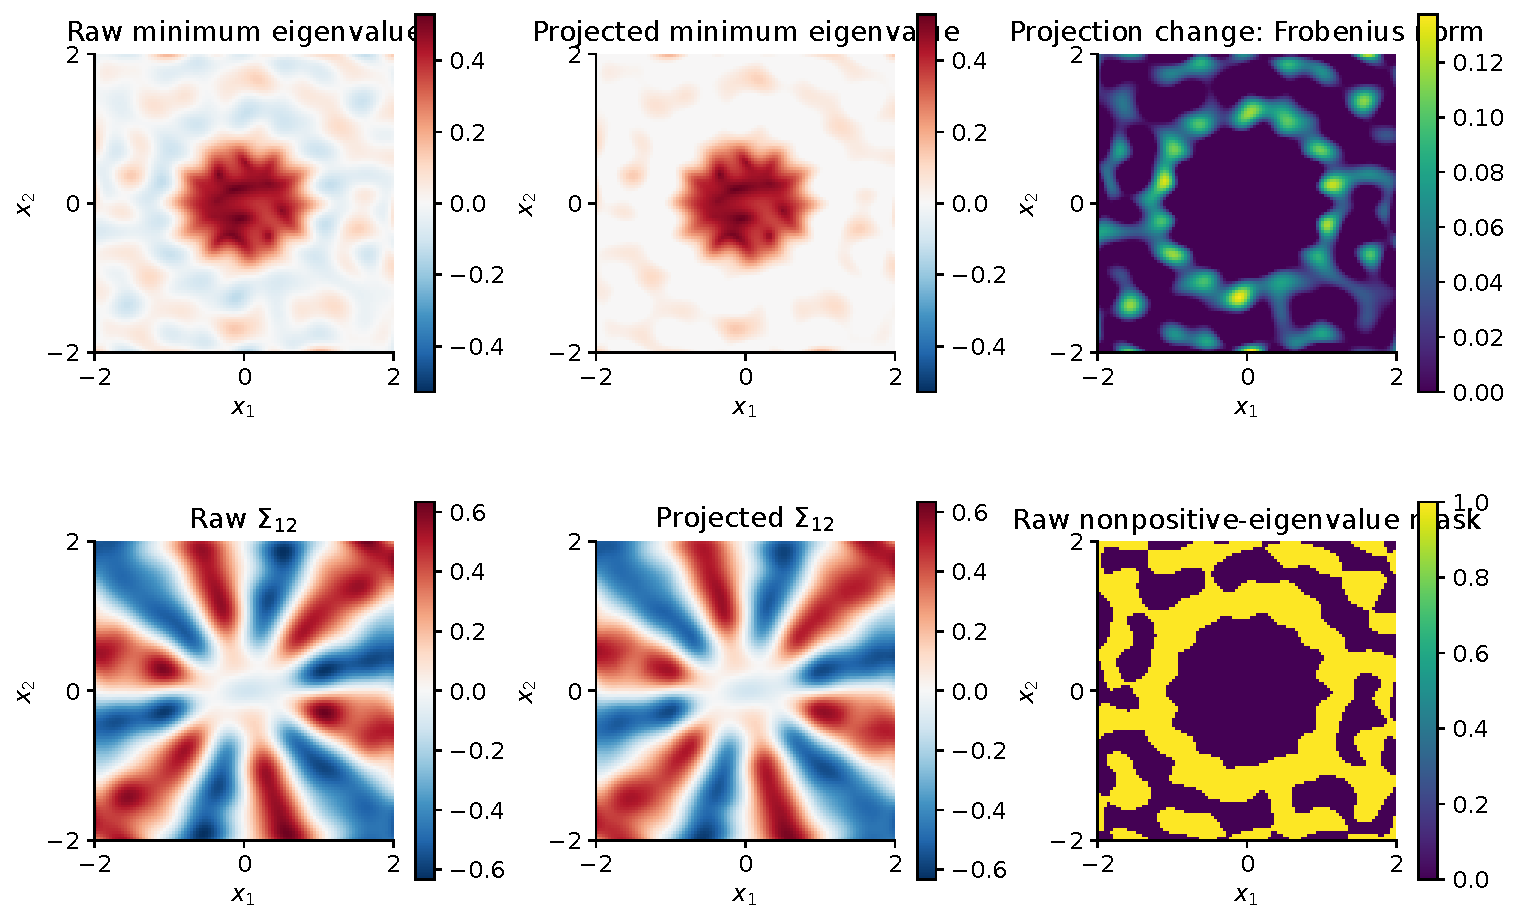
\includegraphics[width=\linewidth]{../figures/ex8_seed0_projection.pdf}
\caption{Seed-0 ARFF: raw and projected smallest eigenvalues, projection-change norm, raw/projected off-diagonal entry, and raw nonpositive-eigenvalue mask. Raw/projected eigenvalue and entry pairs have shared scales. Projection does not repair the raw coefficient estimate retroactively. Grid rates are not the production test-set rates.}\end{figure}

\section{Complete sample-size sensitivity and numerical records}\label{app:sensitivity}
\begin{figure}[htbp]\centering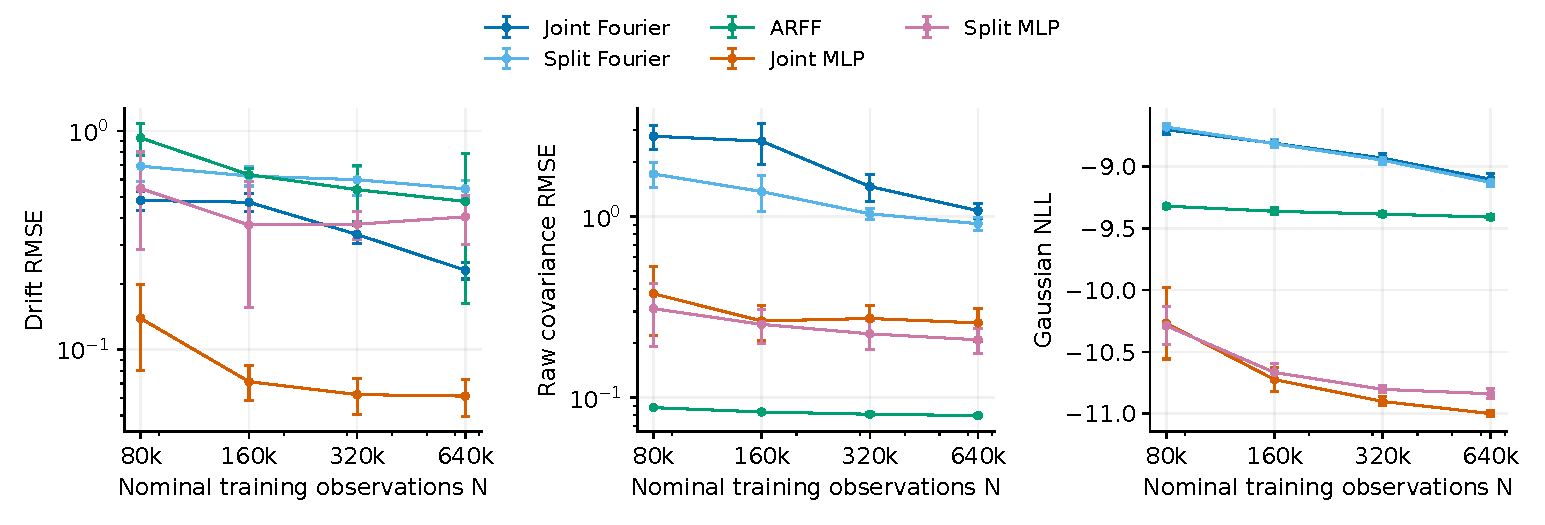
\includegraphics[width=\linewidth]{../figures/N.pdf}\caption{Completed Ex8 sample-size study at $K=1024,h=10^{-4}$: ten fitting seeds on nested training data, with shared validation/test states. Means and sample SDs describe fitting variation, not independent dataset variation.}\end{figure}
The four N points, nine lag points and five capacity points comprise 200,450,250 method/point/seed records, respectively. Their shared 50-record anchor means 800 distinct records, not 900 independent experiments. The 30-seed baseline is separate. Both validation equivalence screens failed; capacity uses the predetermined fallback rather than an established approximation-dominated regime. Full N/h/K and raw-SPD tables follow.
\small
\begin{longtable}{llrrr}\caption{N study: test mean $\pm$ sample SD over ten fitting seeds. Raw covariance errors; all points retained.}\\\toprule Method & Point & Drift RMSE & Raw covariance RMSE & NLL\\\midrule\endfirsthead\toprule Method & Point & Drift RMSE & Raw covariance RMSE & NLL\\\midrule\endhead
Joint Fourier & 80000 & $0.4817\pm 0.0501$ & $2.782\pm 0.4231$ & $-8.704\pm 0.03926$\\
Joint Fourier & 160000 & $0.4723\pm 0.04396$ & $2.613\pm 0.6617$ & $-8.813\pm 0.03376$\\
Joint Fourier & 320000 & $0.3363\pm 0.03173$ & $1.468\pm 0.2504$ & $-8.934\pm 0.03365$\\
Joint Fourier & 640000 & $0.2308\pm 0.02035$ & $1.079\pm 0.1059$ & $-9.105\pm 0.04537$\\
Split Fourier & 80000 & $0.6909\pm 0.1052$ & $1.721\pm 0.2708$ & $-8.682\pm 0.02906$\\
Split Fourier & 160000 & $0.6226\pm 0.06222$ & $1.376\pm 0.3082$ & $-8.817\pm 0.03064$\\
Split Fourier & 320000 & $0.599\pm 0.09298$ & $1.038\pm 0.07346$ & $-8.95\pm 0.0355$\\
Split Fourier & 640000 & $0.5436\pm 0.04761$ & $0.9144\pm 0.07123$ & $-9.13\pm 0.03469$\\
ARFF & 80000 & $0.9297\pm 0.1535$ & $0.08826\pm 0.00116$ & $-9.322\pm 0.01596$\\
ARFF & 160000 & $0.6316\pm 0.04304$ & $0.08352\pm 0.00103$ & $-9.363\pm 0.02774$\\
ARFF & 320000 & $0.5391\pm 0.1531$ & $0.08115\pm 0.0013$ & $-9.386\pm 0.01878$\\
ARFF & 640000 & $0.4763\pm 0.3129$ & $0.07976\pm 0.001234$ & $-9.411\pm 0.01881$\\
Joint MLP & 80000 & $0.1389\pm 0.05881$ & $0.3756\pm 0.1536$ & $-10.27\pm 0.289$\\
Joint MLP & 160000 & $0.07144\pm 0.01292$ & $0.2656\pm 0.0575$ & $-10.72\pm 0.09529$\\
Joint MLP & 320000 & $0.06234\pm 0.01154$ & $0.2742\pm 0.04925$ & $-10.9\pm 0.03649$\\
Joint MLP & 640000 & $0.06135\pm 0.01203$ & $0.2591\pm 0.05327$ & $-11\pm 0.02579$\\
Split MLP & 80000 & $0.5461\pm 0.2588$ & $0.3106\pm 0.118$ & $-10.29\pm 0.1525$\\
Split MLP & 160000 & $0.3719\pm 0.2158$ & $0.2543\pm 0.05389$ & $-10.67\pm 0.06984$\\
Split MLP & 320000 & $0.3749\pm 0.05553$ & $0.2256\pm 0.04057$ & $-10.8\pm 0.02846$\\
Split MLP & 640000 & $0.4052\pm 0.1033$ & $0.209\pm 0.03326$ & $-10.84\pm 0.04174$\\
\bottomrule\end{longtable}
\begin{longtable}{llrrr}\caption{h study: test mean $\pm$ sample SD over ten fitting seeds. Raw covariance errors; all points retained.}\\\toprule Method & Point & Drift RMSE & Raw covariance RMSE & NLL\\\midrule\endfirsthead\toprule Method & Point & Drift RMSE & Raw covariance RMSE & NLL\\\midrule\endhead
Joint Fourier & $2.5\times10^{-5}$ & $0.3259\pm 0.0349$ & $1.507\pm 0.2459$ & $-10.53\pm 0.04815$\\
Joint Fourier & $5\times10^{-5}$ & $0.2687\pm 0.03135$ & $1.273\pm 0.1626$ & $-9.83\pm 0.04447$\\
Joint Fourier & 0.0001 & $0.2308\pm 0.02035$ & $1.079\pm 0.1059$ & $-9.105\pm 0.04537$\\
Joint Fourier & 0.0002 & $0.2049\pm 0.03395$ & $0.9433\pm 0.08391$ & $-8.36\pm 0.04026$\\
Joint Fourier & 0.0004 & $0.139\pm 0.01799$ & $0.8228\pm 0.07923$ & $-7.593\pm 0.041$\\
Joint Fourier & 0.0008 & $0.1389\pm 0.01118$ & $0.7333\pm 0.06999$ & $-6.822\pm 0.03166$\\
Joint Fourier & 0.001 & $0.1393\pm 0.01692$ & $0.6938\pm 0.06811$ & $-6.558\pm 0.02712$\\
Joint Fourier & 0.0015 & $0.1166\pm 0.008672$ & $0.645\pm 0.07429$ & $-6.119\pm 0.02544$\\
Joint Fourier & 0.002 & $0.1032\pm 0.01297$ & $0.6147\pm 0.06438$ & $-5.78\pm 0.01732$\\
Split Fourier & $2.5\times10^{-5}$ & $1.395\pm 0.1083$ & $1.07\pm 0.1096$ & $-10.55\pm 0.03477$\\
Split Fourier & $5\times10^{-5}$ & $0.8385\pm 0.08578$ & $0.9949\pm 0.1184$ & $-9.841\pm 0.04611$\\
Split Fourier & 0.0001 & $0.5436\pm 0.04761$ & $0.9144\pm 0.07123$ & $-9.13\pm 0.03469$\\
Split Fourier & 0.0002 & $0.6084\pm 0.05436$ & $0.818\pm 0.07631$ & $-8.354\pm 0.02488$\\
Split Fourier & 0.0004 & $0.5314\pm 0.07749$ & $0.7129\pm 0.07255$ & $-7.602\pm 0.0304$\\
Split Fourier & 0.0008 & $0.3792\pm 0.04464$ & $0.6297\pm 0.04467$ & $-6.817\pm 0.02917$\\
Split Fourier & 0.001 & $0.3824\pm 0.05917$ & $0.6139\pm 0.03099$ & $-6.542\pm 0.03994$\\
Split Fourier & 0.0015 & $0.3044\pm 0.03002$ & $0.5653\pm 0.02986$ & $-6.11\pm 0.02793$\\
Split Fourier & 0.002 & $0.2632\pm 0.0272$ & $0.5467\pm 0.02664$ & $-5.783\pm 0.03211$\\
ARFF & $2.5\times10^{-5}$ & $0.6348\pm 0.07437$ & $0.07998\pm 0.0008911$ & $-10.81\pm 0.01679$\\
ARFF & $5\times10^{-5}$ & $0.413\pm 0.02228$ & $0.07956\pm 0.001012$ & $-10.12\pm 0.02224$\\
ARFF & 0.0001 & $0.4763\pm 0.3129$ & $0.07976\pm 0.001234$ & $-9.411\pm 0.01881$\\
ARFF & 0.0002 & $0.3425\pm 0.1283$ & $0.07959\pm 0.001313$ & $-8.681\pm 0.02763$\\
ARFF & 0.0004 & $0.2687\pm 0.1031$ & $0.08012\pm 0.001179$ & $-7.93\pm 0.02723$\\
ARFF & 0.0008 & $0.1995\pm 0.1076$ & $0.07953\pm 0.001626$ & $-7.123\pm 0.02359$\\
ARFF & 0.001 & $0.1552\pm 0.06764$ & $0.07934\pm 0.00108$ & $-6.795\pm 0.02148$\\
ARFF & 0.0015 & $0.1115\pm 0.0323$ & $0.07993\pm 0.0009816$ & $-6.196\pm 0.03061$\\
ARFF & 0.002 & $0.08375\pm 0.02096$ & $0.08017\pm 0.001146$ & $-5.766\pm 0.02863$\\
Joint MLP & $2.5\times10^{-5}$ & $0.0603\pm 0.01054$ & $0.3062\pm 0.05858$ & $-12.78\pm 0.0468$\\
Joint MLP & $5\times10^{-5}$ & $0.05781\pm 0.006695$ & $0.2556\pm 0.04349$ & $-11.92\pm 0.02943$\\
Joint MLP & 0.0001 & $0.06135\pm 0.01203$ & $0.2591\pm 0.05327$ & $-11\pm 0.02579$\\
Joint MLP & 0.0002 & $0.05858\pm 0.007052$ & $0.2194\pm 0.01735$ & $-10.05\pm 0.01675$\\
Joint MLP & 0.0004 & $0.05821\pm 0.002943$ & $0.2068\pm 0.02352$ & $-9.071\pm 0.0201$\\
Joint MLP & 0.0008 & $0.05769\pm 0.00288$ & $0.1653\pm 0.01912$ & $-8.083\pm 0.008337$\\
Joint MLP & 0.001 & $0.05743\pm 0.00259$ & $0.1622\pm 0.01598$ & $-7.734\pm 0.01168$\\
Joint MLP & 0.0015 & $0.0606\pm 0.004472$ & $0.1543\pm 0.01148$ & $-7.174\pm 0.0107$\\
Joint MLP & 0.002 & $0.06243\pm 0.00291$ & $0.1351\pm 0.01135$ & $-6.766\pm 0.008771$\\
Split MLP & $2.5\times10^{-5}$ & $0.9113\pm 0.199$ & $0.2537\pm 0.04412$ & $-12.61\pm 0.05613$\\
Split MLP & $5\times10^{-5}$ & $0.5459\pm 0.1921$ & $0.2219\pm 0.03816$ & $-11.78\pm 0.06257$\\
Split MLP & 0.0001 & $0.4052\pm 0.1033$ & $0.209\pm 0.03326$ & $-10.84\pm 0.04174$\\
Split MLP & 0.0002 & $0.445\pm 0.1011$ & $0.1716\pm 0.03286$ & $-9.86\pm 0.05695$\\
Split MLP & 0.0004 & $0.4009\pm 0.0809$ & $0.137\pm 0.01463$ & $-8.89\pm 0.05503$\\
Split MLP & 0.0008 & $0.2219\pm 0.01841$ & $0.1312\pm 0.007079$ & $-7.998\pm 0.02808$\\
Split MLP & 0.001 & $0.1908\pm 0.01301$ & $0.1308\pm 0.01428$ & $-7.657\pm 0.01701$\\
Split MLP & 0.0015 & $0.1631\pm 0.03139$ & $0.1265\pm 0.009742$ & $-7.13\pm 0.01804$\\
Split MLP & 0.002 & $0.1491\pm 0.01474$ & $0.1123\pm 0.01044$ & $-6.724\pm 0.01863$\\
\bottomrule\end{longtable}
\begin{longtable}{llrrr}\caption{capacity study: test mean $\pm$ sample SD over ten fitting seeds. Raw covariance errors; all points retained.}\\\toprule Method & Point & Drift RMSE & Raw covariance RMSE & NLL\\\midrule\endfirsthead\toprule Method & Point & Drift RMSE & Raw covariance RMSE & NLL\\\midrule\endhead
Joint Fourier & 64 & $0.1951\pm 0.06906$ & $0.6597\pm 0.1192$ & $-8.665\pm 0.09647$\\
Joint Fourier & 128 & $0.1555\pm 0.01994$ & $1.085\pm 0.2311$ & $-8.854\pm 0.1013$\\
Joint Fourier & 256 & $0.1427\pm 0.02413$ & $1.661\pm 0.5725$ & $-8.959\pm 0.06919$\\
Joint Fourier & 512 & $0.1598\pm 0.024$ & $1.222\pm 0.2518$ & $-9.047\pm 0.06398$\\
Joint Fourier & 1024 & $0.2308\pm 0.02035$ & $1.079\pm 0.1059$ & $-9.105\pm 0.04537$\\
Split Fourier & 64 & $0.2887\pm 0.02173$ & $0.6717\pm 0.1208$ & $-8.7\pm 0.1052$\\
Split Fourier & 128 & $0.2811\pm 0.0543$ & $0.9447\pm 0.1925$ & $-8.878\pm 0.09829$\\
Split Fourier & 256 & $0.3103\pm 0.05813$ & $1.125\pm 0.2087$ & $-8.974\pm 0.05437$\\
Split Fourier & 512 & $0.4284\pm 0.04236$ & $0.8913\pm 0.1439$ & $-9.061\pm 0.06036$\\
Split Fourier & 1024 & $0.5436\pm 0.04761$ & $0.9144\pm 0.07123$ & $-9.13\pm 0.03469$\\
ARFF & 64 & $0.4629\pm 0.2458$ & $0.1339\pm 0.004343$ & $-8.652\pm 0.1197$\\
ARFF & 128 & $0.5109\pm 0.3023$ & $0.1118\pm 0.003227$ & $-8.961\pm 0.06592$\\
ARFF & 256 & $0.5129\pm 0.2971$ & $0.09663\pm 0.001486$ & $-9.198\pm 0.07232$\\
ARFF & 512 & $0.4642\pm 0.301$ & $0.08692\pm 0.002177$ & $-9.324\pm 0.02425$\\
ARFF & 1024 & $0.4763\pm 0.3129$ & $0.07976\pm 0.001234$ & $-9.411\pm 0.01881$\\
Joint MLP & 64 & $0.2068\pm 0.076$ & $0.2843\pm 0.02909$ & $-10.68\pm 0.1177$\\
Joint MLP & 128 & $0.07759\pm 0.04711$ & $0.2227\pm 0.02277$ & $-10.94\pm 0.04725$\\
Joint MLP & 256 & $0.05875\pm 0.007993$ & $0.2135\pm 0.02941$ & $-10.99\pm 0.02412$\\
Joint MLP & 512 & $0.0564\pm 0.0101$ & $0.2412\pm 0.05395$ & $-11\pm 0.02722$\\
Joint MLP & 1024 & $0.06135\pm 0.01203$ & $0.2591\pm 0.05327$ & $-11\pm 0.02579$\\
Split MLP & 64 & $0.3025\pm 0.08296$ & $0.2354\pm 0.0373$ & $-10.62\pm 0.1642$\\
Split MLP & 128 & $0.3183\pm 0.0657$ & $0.186\pm 0.01817$ & $-10.84\pm 0.05635$\\
Split MLP & 256 & $0.3701\pm 0.07255$ & $0.187\pm 0.01377$ & $-10.88\pm 0.05036$\\
Split MLP & 512 & $0.3993\pm 0.08574$ & $0.1868\pm 0.0206$ & $-10.84\pm 0.0627$\\
Split MLP & 1024 & $0.4052\pm 0.1033$ & $0.209\pm 0.03326$ & $-10.84\pm 0.04174$\\
\bottomrule\end{longtable}
\begin{longtable}{llrr}\caption{Raw ARFF test covariance validity at all sensitivity points. Rate is mean $\pm$ sample SD across ten seeds; minimum eigenvalue is the minimum across all seeds/points. NLL uses the fixed 0.001 floor.}\\\toprule Study & Point & Violation fraction & Minimum eigenvalue\\\midrule\endfirsthead\toprule Study & Point & Violation fraction & Minimum eigenvalue\\\midrule\endhead
N & 80000 & $0.4758\pm 0.007757$ & -0.165507\\
N & 160000 & $0.4807\pm 0.008157$ & -0.141126\\
N & 320000 & $0.4783\pm 0.007681$ & -0.146379\\
N & 640000 & $0.4801\pm 0.006702$ & -0.153866\\
h & $2.5\times10^{-5}$ & $0.4799\pm 0.007949$ & -0.139145\\
h & $5\times10^{-5}$ & $0.4782\pm 0.006613$ & -0.139035\\
h & 0.0001 & $0.4801\pm 0.006702$ & -0.153866\\
h & 0.0002 & $0.4741\pm 0.007878$ & -0.146992\\
h & 0.0004 & $0.4666\pm 0.006847$ & -0.143474\\
h & 0.0008 & $0.4695\pm 0.007821$ & -0.139593\\
h & 0.001 & $0.4665\pm 0.0107$ & -0.143113\\
h & 0.0015 & $0.4562\pm 0.008754$ & -0.141546\\
h & 0.002 & $0.4526\pm 0.007375$ & -0.137715\\
capacity & 64 & $0.4296\pm 0.01529$ & -0.230918\\
capacity & 128 & $0.4509\pm 0.01377$ & -0.177902\\
capacity & 256 & $0.4685\pm 0.008107$ & -0.138869\\
capacity & 512 & $0.4709\pm 0.007596$ & -0.153208\\
capacity & 1024 & $0.4801\pm 0.006702$ & -0.153866\\
\bottomrule\end{longtable}

\normalsize
\subsection{Exploratory lag--drift-ridge intervention}\label{app:lag_ridge}
On corrected Experiment-8 trajectory data, a bounded full-estimator comparison used $K=1024$, nominal $N=640000$, $h\in\{10^{-4},4\times10^{-4},.002\}$, drift ridge $\lambda_f\in\{.001,.008,.064\}$ and fitting seeds 0--2. The nine $\lambda_f=.001$ runs were reused only after data, configuration and source checks; the other 18 fits used the same folds, internal splits and random streams where the native algorithm permits. The penalty changed in all five out-of-fold nuisance drift fits and the final drift fit. The covariance penalty remained $\lambda_\Sigma=.001$, and each covariance fit used its own arm's out-of-fold residual targets. Metropolis updates, 300 adaptations, internal-validation checkpoint selection and no post-selection refit were retained. The final amplitude fits used 576000 observations and each nuisance fit used 460800. These three fitting seeds share one dataset and are not independent-dataset replications. Earlier exploratory decisions had already used the test set, so this is descriptive evidence, not a fresh confirmatory penalty comparison.

\begin{table}[htbp]\centering\small
\caption{All nine lag/ridge arms: test-set means over three fitting seeds on shared data. Earlier exploratory decisions used this test set. Covariance RMSE and SPD violations concern raw predictions; NLL uses the unchanged $10^{-3}$ eigenvalue floor. Lower NLL is better, but its absolute level changes with lag.}
\label{tab:lag_ridge_arms}\resizebox{\linewidth}{!}{\begin{tabular}{llrrrr}
\toprule
$h$ & $\lambda_f$ & Drift RMSE & Raw cov. RMSE & NLL & Raw SPD viol. (\%)\\
\midrule
0.0001 & 0.001 & 0.3714 & 0.0788 & -9.4275 & 48.15\\
0.0001 & 0.008 & 0.3706 & 0.0796 & -9.4166 & 47.50\\
0.0001 & 0.064 & 0.2876 & 0.0785 & -9.4460 & 47.92\\
\addlinespace
0.0004 & 0.001 & 0.2719 & 0.0799 & -7.9312 & 46.04\\
0.0004 & 0.008 & 0.2684 & 0.0798 & -7.9129 & 47.76\\
0.0004 & 0.064 & 0.2175 & 0.0803 & -7.9349 & 46.95\\
\addlinespace
0.002 & 0.001 & 0.0886 & 0.0800 & -5.7442 & 45.18\\
0.002 & 0.008 & 0.0778 & 0.0800 & -5.7617 & 45.85\\
0.002 & 0.064 & 0.0850 & 0.0798 & -5.7477 & 45.33\\
\bottomrule
\end{tabular}
}
\end{table}

\begin{table}[htbp]\centering\small
\caption{Every individual paired test change, intervention minus $\lambda_f=.001$ at the same lag and seed. Negative changes improve the corresponding error or NLL. No seed or valid outcome is omitted.}
\label{tab:lag_ridge_paired}\resizebox{\linewidth}{!}{\begin{tabular}{lllrrr}
\toprule
$h$ & $\lambda_f$ & Seed & $\Delta$ drift RMSE & $\Delta$ raw cov. RMSE & $\Delta$ NLL\\
\midrule
0.0001 & 0.008 & 0 & -0.0258 & -0.00068 & 0.0105\\
0.0001 & 0.008 & 1 & 0.0171 & 0.00120 & -0.0013\\
0.0001 & 0.008 & 2 & 0.0062 & 0.00179 & 0.0236\\
0.0001 & 0.064 & 0 & -0.0485 & -0.00185 & -0.0335\\
0.0001 & 0.064 & 1 & -0.2884 & 0.00037 & -0.0136\\
0.0001 & 0.064 & 2 & 0.0854 & 0.00054 & -0.0084\\
\addlinespace
0.0004 & 0.008 & 0 & -0.0232 & 0.00023 & -0.0245\\
0.0004 & 0.008 & 1 & -0.0100 & -0.00159 & -0.0047\\
0.0004 & 0.008 & 2 & 0.0225 & 0.00101 & 0.0840\\
0.0004 & 0.064 & 0 & -0.0500 & -0.00067 & -0.0276\\
0.0004 & 0.064 & 1 & -0.1153 & -0.00061 & -0.0079\\
0.0004 & 0.064 & 2 & 0.0022 & 0.00247 & 0.0243\\
\addlinespace
0.002 & 0.008 & 0 & -0.0085 & 0.00017 & 0.0451\\
0.002 & 0.008 & 1 & -0.0117 & -0.00063 & -0.1025\\
0.002 & 0.008 & 2 & -0.0124 & 0.00061 & 0.0050\\
0.002 & 0.064 & 0 & -0.0084 & -0.00113 & 0.0353\\
0.002 & 0.064 & 1 & -0.0194 & 0.00022 & -0.0548\\
0.002 & 0.064 & 2 & 0.0170 & 0.00052 & 0.0089\\
\bottomrule
\end{tabular}
}
\end{table}

\begin{figure}[htbp]\centering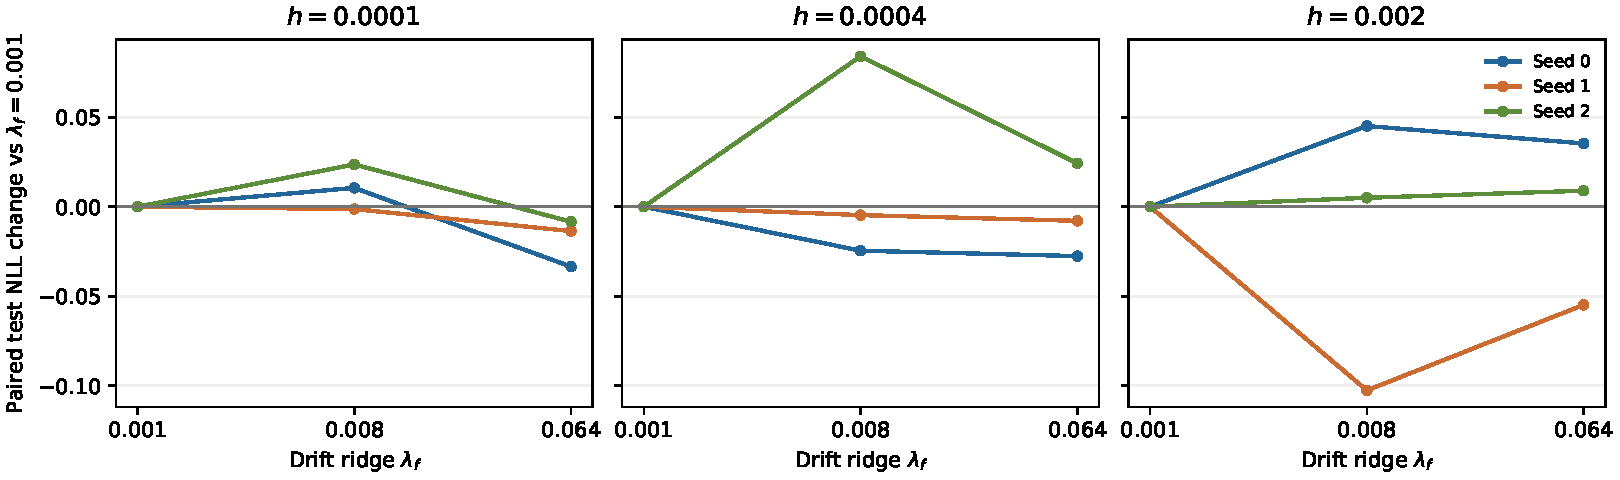
\includegraphics[width=\linewidth]{../figures/lag_ridge_paired_nll.pdf}
\caption{Within-lag paired test NLL changes from $\lambda_f=.001$, with one connected line per fitting seed. The zero at .001 is the same-seed reference, so the lag-dependent density offset does not obscure the intervention. This figure does not select a penalty.}
\label{fig:lag_ridge_nll}\end{figure}

At $h=.002$, $.008$ lowers drift RMSE in all three paired seeds; other drift comparisons are mixed. The larger $.064$ penalty lowers mean drift RMSE at the two shorter lags but worsens one seed at each. Raw covariance RMSE stays near .08 across arms, while raw SPD violations remain common. Paired NLL effects change sign across seeds and lags, except that $.064$ at $h=10^{-4}$ lowers NLL in all three. Final drift checkpoints also change with the penalty; the covariance stage is refitted to each arm's targets. The archived \texttt{per\_run.csv} records all fold/final selected iterations, validation errors, raw minimum eigenvalues and execution scopes. These results do not establish an optimal penalty or a universal benefit, and the ridge intervention was not applied to the production comparisons.

% Proposed appendix after reproducibility appendix. Requires amsmath, graphicx, booktabs.
% Cross-reference from discussion: Appendix~\ref{app:drift_diagnostic}.
\section{A bounded diagnostic of drift estimation error}
\label{app:drift_diagnostic}
This diagnostic explains possible sources of poor drift recovery without changing the production estimator. It uses the Gaussian surrogate
\[
Y=-X+100\sigma(X)\varepsilon,\qquad \varepsilon\sim\mathcal N(0, I_2),
\]
with nominal $h=10^{-4}$, not the canonical finite-lag trajectory data.
The interventions use $N=8192$, fitting subset $n=7373$, $K=1024$ and unnormalized real sine--cosine features. Three algorithm/split repeats share one archived noise pool; they are not three independently generated datasets. Drift MSE averages squared errors over test points and coordinates, and RMSE is its square root per repeat. Expected conditional risk and observed test MSE are distinct quantities.

Condition A freezes frequencies selected with noiseless targets before a noisy amplitude refit. Condition C freezes the first target-independent proposal $\omega_k=0.2Z_k$, $Z_k\sim\mathcal N(0, I_2)$, before target-dependent acceptance. Condition B adapts and selects frequencies using noisy responses. For A/C, exact fixed-design conditional risk separates bias and variance because the frequency choice is independent of the amplitude-fitting noise. That independence does not hold for B.

\begin{table}[ht]
\centering\small
\caption{Means over three paired repeats; distinct risk definitions are not interchangeable. A/C compare $\lambda=.001$ to $.064$. B compares baseline to post-hoc / throughout-path ridge. M/MR both use $\lambda=.064$. Values are rounded only for display.}
\label{tab:drift_diagnostic}
\begin{tabular}{lrrl}\toprule
Comparison & Reference & Intervention & Paired outcome\\\midrule
A: expected conditional MSE & 45.755 & 31.169 & All three improve \\
C: expected conditional MSE & 6.874 & 4.146 & All three improve \\
B: observed test MSE & 16.215 & 9.545 / 10.914 & Post / path ridge \\
M / MR: selected MSE & 10.914 & 6.869 & Two improve, one worsens \\
M / MR: iteration 300 MSE & 124.595 & 616.539 & All three worsen \\
\bottomrule\end{tabular}
\end{table}

For A/C, variance dominates squared bias. Stronger ridge reduces expected and realized error in all six pairs, although the scaled $K=1024$ expected risks remain above their respective $K16$ means (14.607 and 4.017). This is evidence about these bases, not an optimal-ridge rule or a general capacity rate. The normal-equation diagonal shift is $n\lambda$, not $\lambda$.

For B, post-hoc shrinkage on the already selected frequencies reduces observed MSE in all three repeats. Using $.064$ throughout adaptation and checkpoint selection also improves all three relative to baseline, but gives no additional observed benefit over post-hoc shrinkage; repeat 1 is effectively tied (MSE difference $0.000466$). This comparison combines changes to the adaptive path and selection. A noise-independent fixed-basis risk identity cannot be applied to B.

In a separate paired comparison, both arms retain Metropolis updates, $\delta=.2$, $\gamma=1$ and 300 iterations. MR additionally resamples every iteration. The modern update order is proposal, amplitude fit, acceptance, mixed-population refit, optional resampling, and final refit. The earliest strict minimum of noisy internal-validation MSE selects the returned checkpoint; there is no full-data refit. Adding resampling improves two selected models and worsens one. At iteration 300 it worsens all three. The fresh M trajectory is distinct from the archived Bpath trajectory; their close values are not substituted.

\begin{figure}[ht]
\centering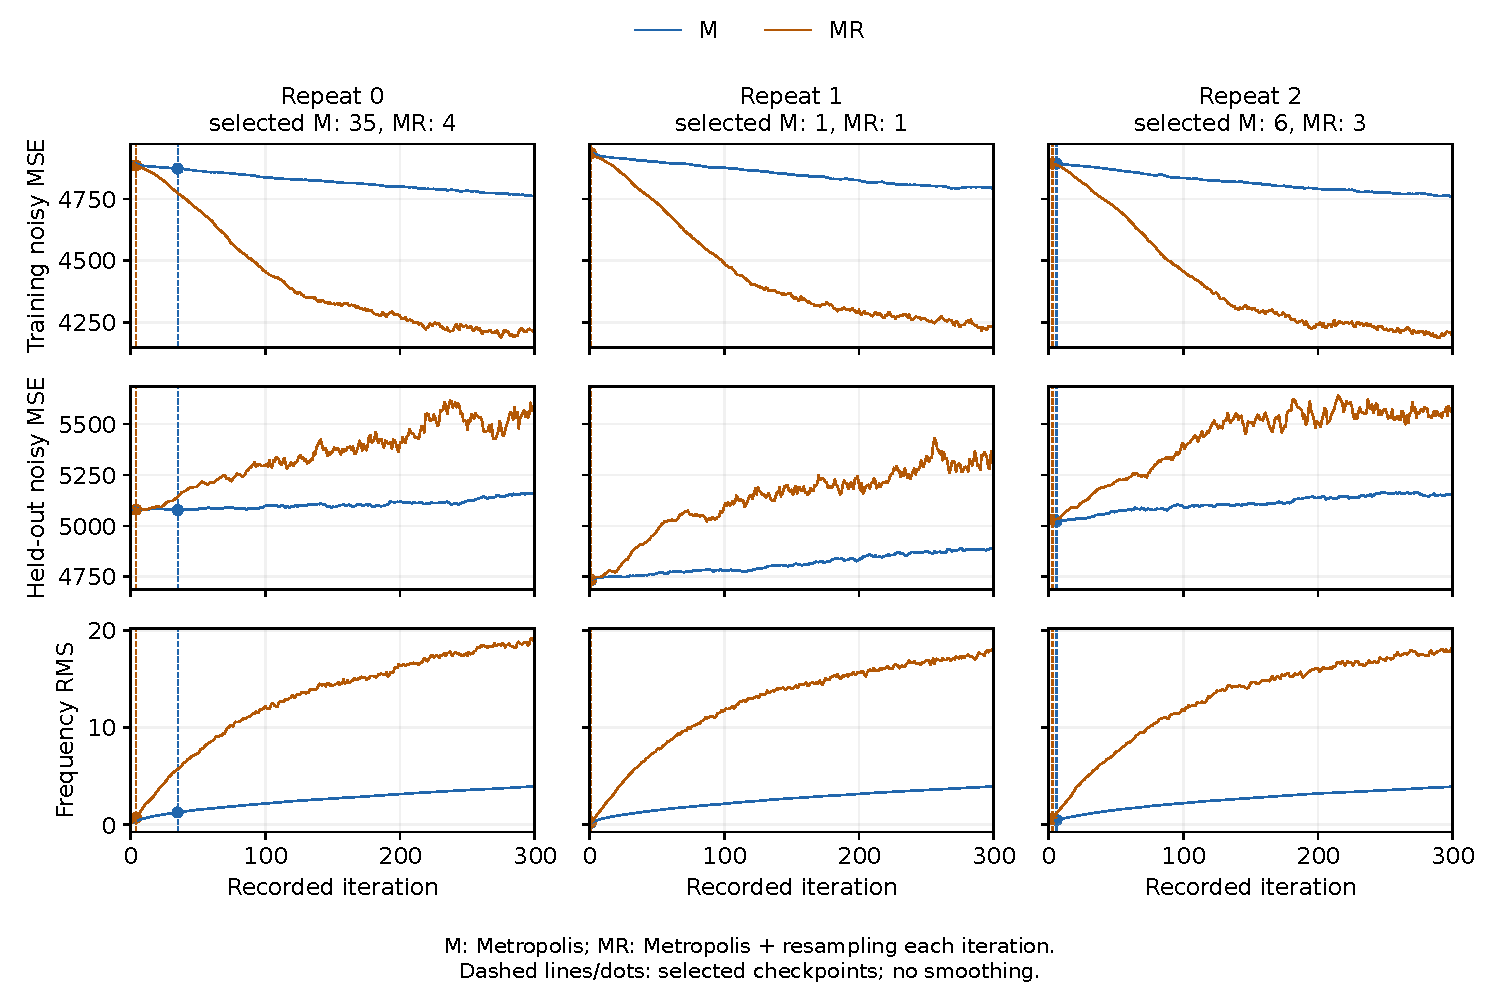
\includegraphics[width=\linewidth]{../figures/mechanism.pdf}
\caption{All recorded training/held-out losses and frequency RMS for all three repeats. Dashed lines and dots mark selected checkpoints. Curves are unsmoothed; frequency RMS includes location as well as spread. Archived centered RMS also grows. No intermediate true-drift errors are inferred.}
\label{fig:drift_diagnostic}
\end{figure}

Training loss decreases overall while held-out noisy loss and frequency spread increase overall; each trajectory has reversals. Selected models have much lower true-drift error than iteration 300. These observations support an overfitting interpretation, but do not prove frequency growth causes it. Noisy checkpoint selection and duplication-induced changes in effective functional regularization remain possible contributors, not isolated causes.

Distinct parent slots are not distinct physical frequencies. Uniform multinomial resampling of 1024 slots already retains only about 647.48 distinct parent slots on average, so observed means near 613 do not establish population collapse. MR's full pre-resampling weights were not archived; ESS alone cannot recover its conditional parent expectation. Higher ESS does not guarantee better recovery.

These results do not establish failure of ESS-triggered resampling, a universal SDE ranking, or an optimal value $.064$. They neither retune the production method nor change production results. The three repeats support these bounded comparisons but do not identify a unique causal mechanism.

\section{Component composition and likelihood calibration}
Post-hoc Joint-MLP-drift/ARFF-covariance composition inherits the component coefficient errors but improves ARFF NLL only modestly. At fixed projected covariance only the quadratic residual term changes. CPU component-swap evaluations are distinct from stored GPU production metrics; float32 and float64 reductions are separate scopes. Their closely rounded values do not denote independent trained models. The instantaneous-coefficient oracle need not optimize finite-lag Gaussian NLL. Fixed-floor sensitivity does not select a replacement production floor.
\begin{table}[ht]\centering\scriptsize\caption{Component-swap CPU evaluations: mean $\pm$ sample SD over 30 seeds. $Q$ is the quadratic term, $D$ the half log-determinant; Gaussian constant $\log(2\pi)=1.837877$. Table~\ref{tab:ex8} instead contains stored production-GPU scores. The float32/float64 blocks agree at four significant digits; paired differences below show their distinct reductions. Identical-oracle roundoff SDs are displayed as zero.}\label{tab:swaps}\begin{tabular}{lrrr}\toprule Combination & $Q$ & $D$ & NLL\\\midrule
\multicolumn{4}{l}{\emph{CPU predictions; float32 projection/likelihood, floor $10^{-3}$}}\\
MLP drift + ARFF cov. & $0.8886\pm 0.0722$ & $-11.64\pm 0.02354$ & $-8.916\pm 0.07438$\\
ARFF drift + ARFF cov. & $0.9074\pm 0.07024$ & $-11.64\pm 0.02354$ & $-8.897\pm 0.07317$\\
True drift + ARFF cov. & $0.8884\pm 0.07218$ & $-11.64\pm 0.02354$ & $-8.916\pm 0.07434$\\
\multicolumn{4}{l}{\emph{CPU predictions; float64 spectral likelihood, floor $10^{-3}$}}\\
MLP drift + ARFF cov. & $0.8886\pm 0.0722$ & $-11.64\pm 0.02354$ & $-8.916\pm 0.07438$\\
ARFF drift + ARFF cov. & $0.9074\pm 0.07024$ & $-11.64\pm 0.02354$ & $-8.897\pm 0.07317$\\
True drift + ARFF cov. & $0.8884\pm 0.07218$ & $-11.64\pm 0.02354$ & $-8.916\pm 0.07434$\\
\multicolumn{4}{l}{\emph{CPU diagnostic; float64, unprojected instantaneous true covariance}}\\
True instantaneous pair & $1.603\times10^{4}\pm 0$ & $-18.42\pm 0$ & $1.602\times10^{4}\pm 0$\\
ARFF drift + true cov. & $1.98\times10^{4}\pm 1947$ & $-18.42\pm 0$ & $1.978\times10^{4}\pm 1947$\\
MLP drift + true cov. & $1.609\times10^{4}\pm 32.45$ & $-18.42\pm 0$ & $1.608\times10^{4}\pm 32.45$\\
\midrule\multicolumn{4}{l}{\emph{Paired CPU float32 minus float64 differences (not new evaluations)}}\\
ARFF drift + ARFF cov. & $-1.609\times10^{-8}\pm 2.323\times10^{-7}$ & $3.116\times10^{-7}\pm 4.146\times10^{-7}$ & $4.112\times10^{-7}\pm 4.87\times10^{-7}$\\
MLP drift + ARFF cov. & $-2.246\times10^{-8}\pm 2.17\times10^{-7}$ & $3.116\times10^{-7}\pm 4.146\times10^{-7}$ & $5.281\times10^{-7}\pm 3.902\times10^{-7}$\\
True drift + ARFF cov. & $-2.537\times10^{-8}\pm 2.306\times10^{-7}$ & $3.116\times10^{-7}\pm 4.146\times10^{-7}$ & $4.795\times10^{-7}\pm 4.794\times10^{-7}$\\
\bottomrule\end{tabular}\end{table}
\begin{table}[ht]\centering\small\caption{Post-hoc float64 floor sensitivity; no floor is selected. All 30 seeds and all prescribed floors retained. Raw covariance RMSE is unchanged. Projected RMSE is shared by the three drift choices.}\begin{tabular}{rrlll}\toprule Floor & Projected cov. RMSE & True drift NLL & MLP drift NLL & ARFF drift NLL\\\midrule
$1\times10^{-8}$ & $0.1129\pm 0.002269$ & $3.327\times10^{4}\pm 6672$ & $3.329\times10^{4}\pm 6673$ & $3.502\times10^{4}\pm 6476$\\
$1\times10^{-6}$ & $0.1129\pm 0.002269$ & $322\pm 66.72$ & $322.2\pm 66.74$ & $339.6\pm 64.77$\\
0.0001 & $0.1129\pm 0.002269$ & $-6.436\pm 0.6757$ & $-6.434\pm 0.6759$ & $-6.258\pm 0.6572$\\
0.001 & $0.1129\pm 0.002269$ & $-8.916\pm 0.07434$ & $-8.916\pm 0.07438$ & $-8.897\pm 0.07317$\\
\bottomrule\end{tabular}\end{table}



\end{document}
